\documentclass[11pt]{article}
\usepackage[margin=1in]{geometry}
\usepackage{amsmath,amssymb,amsthm,mathtools}
\usepackage{booktabs,enumitem,graphicx,xcolor}
\usepackage{xurl}
\usepackage[section]{placeins}
\setlength{\emergencystretch}{3em}
\usepackage[colorlinks=true,linkcolor=blue!50!black,citecolor=green!35!black,urlcolor=blue!50!black]{hyperref}
\usepackage[nameinlink]{cleveref}
\newtheorem{theorem}{Theorem}\newtheorem{proposition}[theorem]{Proposition}\newtheorem{corollary}[theorem]{Corollary}
\newtheorem{lemma}[theorem]{Lemma}
\theoremstyle{definition}\newtheorem{definition}[theorem]{Definition}\newtheorem{remark}[theorem]{Remark}\newtheorem{example}[theorem]{Example}
\newcommand{\R}{\mathbb R}
\newcommand{\Bern}{\mathrm{Bern}}
\DeclareMathOperator{\rank}{rank}\DeclareMathOperator{\im}{im}\DeclareMathOperator{\coker}{coker}\DeclareMathOperator{\Spec}{Spec}

\title{Partial Gluing and Level Two:\\ Graded Explanations, Latent Actors and Paths through Singularities}
\author{Vinay K Awasthi\\ Johns Hopkins University\\ \texttt{vawasth1@jh.edu}}
\date{October 2026}

\begin{document}
\maketitle

\begin{abstract}
When local tables of evidence fail to glue into one global law, the usual response is to stop. We stay at the failure and ask how much
structure can still be saved. For a family of tables with noncontextual fraction $\lambda^*<1$, the laws that account for a fraction
$\alpha$ of every table form a polytope $E_\alpha$. It is non-empty exactly when $\alpha\le\lambda^*$, it shrinks as $\alpha$ grows, and
its prediction intervals and its maximum-entropy member move continuously with $\alpha$. The gradation $\alpha$ is how much of the gluing
we keep; the rest, $1-\alpha$ of every table, is mass we let dissipate. We then go up one level, to laws over hypotheses: latent types of
patients (actors) whose mixture produces the observed law. The explanations at this level are the real points of the fibre of a
polynomial map, an affine scheme, and its geometry carries what happens to the actors. Where two types coincide the fibre is singular, a
second-order obstruction $\kappa$ (the first non-abelian term, $\ell_2\neq 0$) is non-zero, and the tangent cone is a union of planes:
types can split apart along one variable for free but not along two. Along a straight path of observed laws the types separate like
$\sqrt{s}$ (two Puiseux branches); on the other side of the independence locus the two explanations become complex conjugates, no real
two-type explanation exists, and a third type is needed. Going around a loop of populations can exchange the roles of the two actors ($\mathbb Z/2$ monodromy). With three measured
variables this exchange must pass through a singularity; with four it need not. We illustrate everything on a drug-combination problem:
baseline and single-drug harms are known, pairs have been trialled, the triple combination has not. Latent types narrow the prediction
interval about fivefold; when the pair trials conflict, the graded explanations say what can be predicted when 20\%, 40\%, 70\% or 86\%
of the structure is saved. Finally we make the scheme structure explicit. In mean-and-difference coordinates the model is a toric family
over the weights; the fibre over an independent law is exactly the Stanley--Reisner scheme of a small simplicial complex whose faces are the
strata (it is reduced); and for three variables the model inverts in closed form, flatness fails exactly where an actor is absent or the
actors agree on a variable, and the sign of Cayley's hyperdeterminant separates genuine mixtures, signed mixtures and complex-conjugate
pairs. Real explanations can vanish only at a wall of the parameter box or at the non-flat locus, and this is why role exchange needs a
singularity with three variables but not with four. Both levels then sit on one ladder of base semirings, $\mathbb C\supset\R\supset
\R_{\ge0}$: disagreement on an overlap has no points at all; contextuality has real points but no positive ones, with negativity comparable
to $1-\lambda^*$; and at level two a further rung of complex-conjugate actors appears. Finally we let the coefficients be matrices and
keep what fails to commute: commutators decide the cover of contexts (CHSH gives $\lambda^*=2-\sqrt2$), order effects are bounded by
commutator norms, the canonical Kirkwood--Dirac section puts the commutation obstruction on the complex rung, loops carry a geometric
phase that becomes non-abelian with rank-two projections, and non-commuting projections steer a state along a probability path (Zeno
dragging) where commuting ones cannot. With the measurements given but partly masked, the linear fit locates a hidden direction exactly
when the known directions on its side span space, leaving otherwise a linear ambiguity of computable dimension; positivity then culls the
candidates that would imply negative probabilities, and what remains recoverable are the invariants of the residual symmetry. Last, quantum
graded gluing is the positivity domain of a hereditary quadratic matrix polynomial in the sense of Islam, Volčič and Woerdeman: its walls are
determinantal free loci, and the quantum fraction lies below the classical fraction of every product-basis view, with equality for classical
data and for pairwise Werner windows, where it exhibits monogamy. A final section gives these pieces a common categorical home: the contexts
are a diagram of commutative subalgebras and contextuality a failed limit over it (Kochen--Specker versus Gleason, exact on the Peres--Mermin
square); representation functors explain the gauge and show that a holonomy phase $q$ allows finite dimension only when $q^n=1$; positivity on
truncated free modules (NPA) gives the quantum rung without fixing a dimension, with closed forms on isotropic boxes; and divergence-enriched
categories give a data processing inequality for $\lambda^*$. All claims are checked: nine numerical checks (\texttt{engine/check\_level2.py})
six exact symbolic ones (\texttt{engine/check\_scheme.py}), six on the ladder
(\texttt{engine/check\_ladder.py}) eight on non-commutativity (\texttt{engine/check\_noncomm.py}) seven on masked measurements
(\texttt{engine/check\_masked.py}, \texttt{engine/check\_masked\_gauge.py}) six on quantum graded gluing (\texttt{engine/check\_qglue.py}) and six on the categorical home (\texttt{engine/check\_npa.py}).
\end{abstract}

\section{The problem: a combination nobody has trialled}\label{sec:problem}

Three drugs $A,B,C$ are each known by themselves: single-drug trials give the rate of harm under each. Pairs have been trialled: from the
$AB$, $BC$ and $AC$ trials we have the joint tables of harm. The triple combination has not been given to anyone. Write $H_A,H_B,H_C\in
\{0,1\}$ for whether a patient is susceptible to the harm of each drug, and suppose for the illustration that a patient on a combination
is harmed when susceptible to at least one of its drugs. The question is
\[
  P(\text{any harm}\mid A{+}B{+}C) \;=\; 1-P(H_A=H_B=H_C=0),
\]
a property of the joint law of $(H_A,H_B,H_C)$, which no trial has observed. The baseline (no drug, no harm) and the single-drug margins are
the known blobs; the joint law is the unknown blob; the pair tables are \emph{windows} onto it.

Three things can happen.
\begin{enumerate}[leftmargin=*,itemsep=2pt]
\item The pair tables glue, and the set of global laws consistent with them gives an interval for the triple harm (level one).
\item Patients come in latent types, actors that are invisible in the data but shape it: a type susceptible to $A$ and $C$, say, and a
type susceptible to $B$. The same patient can play different roles in different pairs. If we are willing to assume a small number of types,
the interval narrows (level two, \cref{sec:level2}).
\item The pair tables do not glue: the $BC$ trial was run in a different population. The standard answer is that there is no global
law and nothing to predict. We stay at the failure and grade it (\cref{sec:graded}).
\end{enumerate}
The rest of the note develops each, and then follows the latent actors through the singular places of their geometry: where they merge,
where one of them disappears, where a new one must be born, and where they exchange roles.

\section{Sitting at the gluing failure: graded explanations}\label{sec:graded}

Let $X=(X_v)_{v\in V}$ take values in finite sets, and let a family of windows $w$ have scopes $S_w\subseteq V$ and tables $t_w$, laws on
the values of $X_{S_w}$. For a law $q$ on the values of $X$ write $q|_w$ for its marginal on $S_w$. The \emph{noncontextual fraction}
\cite{AbramskyBarbosaMansfield2017} is
\[
  \lambda^* \;=\; \max\{\,\mu(\text{all}) : \mu\ge 0 \text{ a measure on the values of } X,\ \mu|_w\le t_w \text{ for every } w\,\},
\]
a linear program. The tables glue (there is a global law with these marginals) iff $\lambda^*=1$.

\begin{definition}[graded explanation]
For $\alpha\in(0,1]$, an \emph{$\alpha$-explanation} is a law $q$ with $\alpha\, q|_w\le t_w$ for every window. Write $E_\alpha$ for the
set of them. For an event $F$, the \emph{$\alpha$-prediction interval} is $[\min_{q\in E_\alpha} q(F),\ \max_{q\in E_\alpha}q(F)]$
(two linear programs), and the \emph{most probable explanation} $q_\alpha$ is the maximiser of the entropy $H(q)$ over $E_\alpha$.
\end{definition}

An $\alpha$-explanation splits every table in two,
\begin{equation}\label{eq:split}
  t_w \;=\; \alpha\, q|_w \;+\; (1-\alpha)\, r_w, \qquad r_w=\frac{t_w-\alpha q|_w}{1-\alpha}\ \text{ a law on } S_w ,
\end{equation}
a part $\alpha q|_w$ that comes from one global law, and a residue $r_w$ that comes from no common source: the residues of different windows
need not agree on their overlaps. The fraction $\alpha$ is the structure we save; $1-\alpha$ of the mass of every table is let go. This is
the gradation in gluing.

\begin{proposition}\label{prop:graded}
\begin{enumerate}[label=(\roman*),leftmargin=*,itemsep=1pt]
\item $E_\alpha\neq\emptyset$ iff $\alpha\le\lambda^*$.
\item If $\alpha\le\beta$ then $E_\beta\subseteq E_\alpha$. Hence prediction intervals are nested: saving more structure never widens
them.
\item On $(0,\lambda^*]$ the map $\alpha\mapsto E_\alpha$ is continuous (in the Hausdorff metric), and so are the endpoints of every
prediction interval and the most probable explanation $q_\alpha$, which is unique.
\item If all table entries are positive, $E_\alpha$ is the whole simplex for small $\alpha$: the interval is $[0,1]$ for any event that is
neither sure nor impossible, and $q_\alpha$ is the uniform law.
\end{enumerate}
\end{proposition}

\begin{proof}
(i) If $q\in E_\alpha$ then $\mu=\alpha q$ is feasible for the program defining $\lambda^*$ with total mass $\alpha$, so $\alpha\le
\lambda^*$. Conversely, if $\mu$ attains $\lambda^*$ and $\alpha\le\lambda^*$, then $q=\mu/\lambda^*$ satisfies $\alpha q|_w\le
\lambda^* q|_w=\mu|_w\le t_w$. (ii) $\alpha q|_w\le\beta q|_w\le t_w$.
(iii) Let $M=\{\mu\ge0:\mu|_w\le t_w\}$, a convex polytope; $E_\alpha=\{\mu/\alpha:\mu\in M,\ \mu(\text{all})=\alpha\}$. The correspondence $\alpha\mapsto E_\alpha$ has a closed graph and compact values, so it is upper hemicontinuous. It is also lower hemicontinuous: given $q\in E_\alpha$ and $\alpha_n\to\alpha$, if $\alpha_n\le\alpha$ then $q\in E_{\alpha_n}$ by (ii); if $\alpha<\alpha_n\le\lambda^*$, take $\mu^*\in M$ of mass $\lambda^*$ and $s_n\to0$ with $(1-s_n)\alpha+s_n\lambda^*=\alpha_n$; then $\mu_n=(1-s_n)\alpha q+s_n\mu^*\in M$ (by convexity) has mass $\alpha_n$, and $q_n=\mu_n/\alpha_n\in E_{\alpha_n}$ tends to $q$. A continuous compact-valued correspondence has continuous maxima and minima of a
continuous function (Berge's maximum theorem \cite{Berge1963}); the entropy is strictly concave, so its maximiser is unique and
continuous. (iv) If every entry of every table is positive, every law $q$ satisfies $\alpha q|_w\le t_w$ once $\alpha\le\min t_w$, so $E_\alpha$ is the whole simplex for small $\alpha$; zero entries in the tables force the corresponding cells to zero for every $\alpha$, and the statement holds on the remaining face.
\end{proof}

So the graded explanations form a path. At $\alpha\to0$ we have saved nothing and know nothing; at $\alpha=\lambda^*$ we have saved all
the structure that can be saved together. In between, $\alpha\mapsto q_\alpha$ is the \emph{most probable path} from ignorance to the
best partial gluing, and the prediction band around it narrows monotonically.

\begin{example}[conflicting pair trials]\label{ex:conflict}
Let the truth in population~1 be two patient types with weights $(0.6,0.4)$ and susceptibilities
\[
  a_1=(0.5,\ 0.1,\ 0.4),\qquad a_2=(0.05,\ 0.5,\ 0.1)\qquad(\text{for }H_A,H_B,H_C),
\]
the harms independent within a type. The $AB$ and $AC$ trials sample population~1; the $BC$ trial samples population~2, with the same
types in proportions $(0.25,0.75)$. Each table is exact, but together they do not glue: $\lambda^*=0.86$. The triple-combination harm is
$0.667$ in population~1 and $0.612$ in population~2. \Cref{tab:graded} and \cref{fig:main}(a) show the graded answer.
\end{example}

\begin{table}[!htbp]\centering\small
\begin{tabular}{cccp{0.36\linewidth}}\toprule
structure saved $\alpha$ & prediction interval & most probable $q_\alpha$ & reading\\\midrule
$0.2$ & $[0,\,1]$ & $0.867$ & nothing ruled out; close to the uniform law ($7/8$)\\
$0.4$ & $[0,\,1]$ & $0.835$ & \\
$0.6$ & $[0.233,\,0.976]$ & $0.781$ & the trials begin to bite\\
$0.7$ & $[0.343,\,0.836]$ & $0.765$ & \\
$0.8$ & $[0.488,\,0.732]$ & $0.694$ & \\
$0.86=\lambda^*$ & $[0.594,\,0.681]$ & $0.647$ & all that can be saved; both populations' truths inside\\
$0.87$ & none & none & cannot be saved together\\\bottomrule
\end{tabular}
\caption{Graded partial gluing of the conflicting pair trials (\cref{ex:conflict}): the triple-combination harm when a fraction
$\alpha$ of every table is explained by one global law and $1-\alpha$ is let go.}\label{tab:graded}
\end{table}

At $\alpha=\lambda^*$ the interval $[0.594,0.681]$ contains the triple harm of both populations. This is not a theorem (it is a
property of this example), but it shows what the graded answer is for: when the evidence conflicts, the interval at the largest
savable fraction is an honest statement of what is still predictable, and the residues $r_w$ in \eqref{eq:split} say where the
conflict lives.

\section{Level two: latent actors}\label{sec:level2}

Level one asks for a law on outcomes. Level two asks for a law on hypotheses that produces it: here, a mixture of patient types.

\begin{definition}[latent class model]
With $k$ types and $m$ binary variables, type $h$ has weight $w_h$ and susceptibilities $a_h\in[0,1]^m$, the variables independent given
the type. The observed law is
\[
  F(w,a) \;=\; \sum_{h=1}^k w_h\,\Pi(a_h),\qquad \Pi(a_h)=\Bern(a_{h1})\otimes\cdots\otimes\Bern(a_{hm}),
\]
a polynomial map from $\Delta_{k-1}\times[0,1]^{km}$ to the simplex of laws on $\{0,1\}^m$.
\end{definition}

For an observed law $P$, the level-two explanations are the real points, with $w\ge0$ and $a\in[0,1]^{km}$, of
\[
  \mathcal X_P \;=\; \Spec\ \R[w,a]\big/\big(\textstyle\sum_h w_h-1,\ F(w,a)-P\big),
\]
the fibre of $F$ over $P$, an affine scheme. When only windows are observed, $F$ is composed with the marginal maps, and the fibre is
taken over the observed tables. Level one is the image; level two is the fibre. Everything that happens to the actors happens in the
fibre: a fibre that is a finite set of points (identification), a curve (a one-parameter family of explanations), a point where two
branches cross (actors that merge), or empty (no explanation with this many actors).

For $k=2$ and $m=3$ there are $1+2m=7$ parameters and the laws on $\{0,1\}^3$ form a 7-dimensional simplex; generically the fibre over
the full law is two points, exchanged by swapping the labels of the types \cite{AllmanMatiasRhodes2009}. Over the three pair tables
(6 numbers after normalisation) the fibre is a curve.

\begin{example}[latent structure sharpens prediction]\label{ex:sharpen}
In population~1 of \cref{ex:conflict}, with all three pair trials run there, the pair tables glue. Level one (any global law with these
pair tables) gives the triple harm in $[0.654,\,0.694]$. Level two (any mixture of two types with these pair tables) gives
$[0.6613,\,0.6687]$, about five times narrower, and still containing the truth $0.667$ (\cref{fig:main}(b)). The level-two interval was
computed by tracing the fibre curve: we fix $w_1$ on a grid of 49 values and solve for the susceptibilities from 12 starts each; 228
exact solutions were found.
\end{example}

Assuming latent actors is a modelling choice and the narrower interval is only as good as that choice. What the fibre adds is that the
choice is explicit and its consequences can be computed, including where it breaks.

\paragraph{Graded gluing at level two.}
The gradation of \cref{sec:graded} lifts: the level-two gluable fraction is
\[
  \lambda^*_2 \;=\; \sup\{\alpha:\ \alpha\,F(w,a)|_w\le t_w \text{ for every window, for some } (w,a)\},
\]
the largest share of every table that a $k$-type population can account for. Since $F(w,a)$ is a law, $\lambda_2^*\le\lambda^*$. For the
conflicting trials of \cref{ex:conflict} the best two-type explanation found saves $0.86$, the same as level one: there, assuming two
actors costs no structure. Unlike $\lambda^*$, $\lambda^*_2$ is not a linear program (it is a polynomial optimisation), and the values we
report are the best found from many starts, so they are lower bounds.

\section{Singularities and the second-order obstruction}\label{sec:singular}

Let $J=dF$ at a point $x=(w,a)$, restricted to directions with $\sum_h\delta w_h=0$, and viewed as a map into the sum-zero directions of
the simplex. Its kernel $K$ is the space of first-order deformations of the explanation that leave the observed law unchanged; let $C$ be
a basis of its cokernel. Define the \emph{second-order obstruction}
\[
  \kappa(v) \;=\; C^{\!\top} D^2F(v,v),\qquad v\in K.
\]

\begin{proposition}[Kuranishi test \cite{Kuranishi1962}]\label{prop:kur}
If $\gamma(t)$ is a smooth path in the fibre with $\gamma(0)=x$ and $\gamma'(0)=v$, then $v\in K$ and $\kappa(v)=0$.
\end{proposition}

\begin{proof}
Differentiate $F(\gamma(t))=P$ twice at $t=0$: $J v=0$ and $J\gamma''(0)+D^2F(v,v)=0$, so $D^2F(v,v)\in\im J$, which $C^{\!\top}$
annihilates.
\end{proof}

At a regular point $K=0$ and nothing is obstructed. The obstruction is the first term of the deformation problem that is not linear:
in the language of $L_\infty$ algebras \cite{LadaStasheff1993} it is the bracket $\ell_2$, and at level one (where the explanation sets are polytopes) it
vanishes identically. Level two is where it first appears. The fibre has three kinds of points (\cref{tab:strata}).

\begin{table}[!htbp]\centering\small
\begin{tabular}{llccl}\toprule
point & meaning & $\rank J$ & $\dim K$ & obstruction\\\midrule
generic & two distinct, present actors & $2m+1=7$ & 0 & none\\
$w_2=0$ & an actor absent & $m+1=4$ & $m=3$ & $\kappa=0$: its role is free\\
$a_1=a_2$ & two actors coincide & $m=3$ & $m+1=4$ & $\kappa\neq 0$ off a union of planes\\\bottomrule
\end{tabular}
\caption{Strata of the two-type, three-variable fibre ($m=3$). An absent actor can take any role at no cost; coinciding actors can be
pulled apart only along special directions.}\label{tab:strata}
\end{table}

\begin{theorem}[tangent cone at a coincidence]\label{thm:cone}
Let $a_1=a_2=c\in(0,1)^m$ and $w\in(0,1)^2$. The kernel $K$ is spanned by the weight direction $(\delta w,0)$ with $\delta w=(1,-1)$ and the
\emph{splits} $s(e)=(0;\ -\tfrac{w_2}{w_1}e,\ e)$, $e\in\R^m$. For $v=t\,(\delta w,0)+s(e)$,
\[
  \kappa(v) \;=\; \frac{2w_2}{w_1}\sum_{i<j} e_ie_j\; C^{\!\top}\partial_{ij}\Pi(c),
\]
which vanishes iff $e$ has at most one non-zero coordinate. The tangent cone of the fibre at the coincidence is therefore the union of
the $m$ planes $\langle(\delta w,0),\, s(\mathbf e_i)\rangle$, which meet along the weight line, and each plane is filled by exact paths in the
fibre.
\end{theorem}

\begin{proof}
Write $\partial_S\Pi(c)$ for $\Pi$ with the factors $i\in S$ replaced by $(-1,1)$. The $2^m$ vectors $\partial_S\Pi(c)$ form a basis
(a tensor product of bases $\{\Bern(c_i),(-1,1)\}$), and those with $S\neq\emptyset$ span the sum-zero directions. The columns of $J$ are
$\Pi(a_1)-\Pi(a_2)=0$ (weights) and $w_h\partial_i\Pi(c)$ (susceptibilities), so $\im J=\langle\partial_i\Pi\rangle$, the kernel is as
stated, and the cokernel is spanned by $\partial_S\Pi$ with $|S|\ge2$. In $D^2F(v,v)=2\sum_h\sum_i\delta w_h\delta a_{hi}\partial_i\Pi+
2\sum_h w_h\sum_{i<j}\delta a_{hi}\delta a_{hj}\partial_{ij}\Pi$ (there are no $\partial_{ii}$ terms, $F$ being multilinear in each
$a_h$), the first sum lies in $\im J$ and the second equals $2\big(w_1\tfrac{w_2^2}{w_1^2}+w_2\big)\sum_{i<j}e_ie_j\partial_{ij}\Pi=
\tfrac{2w_2}{w_1}\sum_{i<j}e_ie_j\partial_{ij}\Pi$. Since the $\partial_{ij}\Pi$ are independent modulo $\im J$, $\kappa(v)=0$ iff
$e_ie_j=0$ for all $i<j$. For the paths: if two types differ only in variable $i$, the mixture is still a product law, whose $i$-th margin is
$w_1a_{1i}+w_2a_{2i}$; moving the weights and spreading $a_{1i},a_{2i}$ while keeping this mean fixed stays in the fibre exactly.
\end{proof}

A mixture of two products that differ in one variable is itself a product. Actors that differ in only one respect are therefore
invisible: the fibre contains a whole plane of them through the coincidence. Actors that differ in two respects or more create a
correlation, and they cannot be separated infinitesimally without changing the observed law at second order. \Cref{fig:main}(d) shows
$|\kappa|$ around the circle of splits in the $(X_1,X_2)$ plane: it vanishes exactly on the two coordinate axes and is proportional to
$|\sin2\varphi|$ in between.

\section{Where mass dissipates: paths through singularities}\label{sec:puiseux}

Now move the observed law. Fix $w=(\tfrac12,\tfrac12)$, $c\in(0,1)^3$ and $e\in\R^3$ with all $e_i\neq0$, and set $B=\sum_{i<j}e_ie_j
\,\partial_{ij}\Pi(c)$ and $P(s)=\Pi(c)+sB$, a straight line of laws through the product law $\Pi(c)$.

\begin{theorem}[two branches, then none]\label{thm:puiseux}
\begin{enumerate}[label=(\roman*),leftmargin=*,itemsep=1pt]
\item For $s>0$ (small enough that the parameters stay in $[0,1]$), $P(s)=F\big(w,\ (c+\sqrt s\,e,\ c-\sqrt s\,e)\big)$ exactly. The two
types separate like $\sqrt s$, and the two Puiseux branches $\pm\sqrt s$ \cite{CasasAlvero2000} are exchanged by swapping labels.
\item For $s<0$ no mixture of two (or one) product laws equals $P(s)$.
\item At $s=0$ the path passes through the coincidence stratum of \cref{thm:cone}.
\end{enumerate}
\end{theorem}

\begin{proof}
(i) $\Pi(c+te)=\sum_S t^{|S|}e_S\,\partial_S\Pi(c)$ with $e_S=\prod_{i\in S}e_i$. The average of $t$ and $-t$ keeps the even terms:
$\Pi(c)+t^2B$ for $m=3$. Put $t^2=s$.
(ii) Under $P(s)$ the covariance of $X_i,X_j$ is $s\,e_ie_j$, so the product of the three pairwise covariances is $s^3(e_1e_2e_3)^2<0$.
Under any two-type law it is $\prod_{i<j}w_1w_2d_id_j=(w_1w_2)^3(d_1d_2d_3)^2\ge0$, where $d=a_1-a_2$.
\end{proof}

This is the precise form of an abrupt change. The observed law moves linearly in $s$; the explanation moves like $\sqrt s$, with
infinite speed at $s=0$; and on the far side the two-type structure is gone from the real world: the same formula gives
$c\pm i\sqrt{|s|}\,e$, a complex-conjugate pair of explanations (\cref{sec:scheme} makes this exact). In the space of observed laws the image of $F$ has a fold
along the independence locus, and the path crosses it. \Cref{fig:main}(c) shows the gap $\max_i|a_{1i}-a_{2i}|=2\sqrt s\max_i|e_i|$ fitted
from the data, exactly on the curve, and the best two-type misfit for $s<0$: $0.0004$, $0.0008$, $0.0017$ and $0.0035$ at
$s=-0.005,-0.01,-0.02,-0.04$.

Graded gluing says how much is lost. Beyond the fold $\lambda^*_2<1$: some mass of every observed law must be let go if two actors are to
explain the rest. The best two-type explanations we found save $0.9990$, $0.9926$, $0.9960$, $0.9919$ and $0.9836$ of the structure at $s=-0.0025$, $-0.005$, $-0.01$, $-0.02$, $-0.04$: about $1\%$ of the mass must go, a little more as $s$ moves away from the fold. These are attained values and so lower bounds on $\lambda^*_2$; that they are not monotone in $s$ shows the optimiser does not resolve the exact rate. The mass does not vanish into nothing, however: three
types fit $P(s)$ exactly for $s=-0.01$ and $s=-0.04$ (residual below $10^{-14}$). What dissipates is the two-actor organisation of the
mass, and what is born on the far side is a third actor. Read in the other direction, the fold is where a type dies: as $s\downarrow0$
the two types merge, and their difference, which had carried a correlation, becomes a free direction of the kind in \cref{tab:strata}.

\section{Dual roles and monodromy}\label{sec:monodromy}

The labels ``type~1'' and ``type~2'' are not in the data. Over a generic law the fibre is two points that differ only in the labels, and
along a path of laws the labels can be carried by continuity. Around a closed loop of laws they may come back exchanged: the actor that
played the $A$-susceptible role now plays the $B$-susceptible one. This is the monodromy of the map $F$, here a subgroup of $\mathbb Z/2$
(of the symmetric group $S_k$ for $k$ types).

We build such loops explicitly. With a centre $c$, directions $u,v\in\R^m$, $r=0.22$ and $\rho=0.15$, put
\[
  a_{1,2}(\theta)=c\pm r(\cos\theta\,u+\sin\theta\,v),\qquad w(\theta)=\big(\tfrac12+\rho\cos\theta,\ \tfrac12-\rho\cos\theta\big),
  \qquad\theta\in[0,\pi].
\]
At $\theta=\pi$ the parameters are those at $\theta=0$ with the labels swapped, so the observed law $F(\theta)$ returns to its start (to
$10^{-12}$): a half circle of parameters is a closed loop of observed laws, and tracking the explanation along it exchanges the actors.

\begin{theorem}[three variables force a singularity]\label{thm:m3}
Let $m=3$, $k=2$. Any continuous path of parameters with $w\in(0,1)^2$ from $(w,a_1,a_2)$, with all $d_i=a_{1i}-a_{2i}\neq0$, to its
relabelling $(w_2,w_1,a_2,a_1)$ passes, for each variable $i$, through a point where $d_i=0$, and there $\rank J\le5<7$.
So within the regular locus no role exchange is possible.
\end{theorem}

\begin{proof}
Along the path $d_i$ goes from $d_i$ to $-d_i$ and so vanishes somewhere. Where $d_3=0$, say, the law is $G(w,a_{\cdot,1:2})\otimes
\Bern(c_3)$, where $G$ is the two-type model on the first two variables. $G$ has $5$ parameters and a $3$-dimensional target, so its
differential has a kernel of dimension at least $2$; those directions (with $\delta a_{\cdot3}=0$) are in the kernel of $J$.
\end{proof}

With four variables the same argument leaves a two-type model on three variables, which is generically regular, and nothing forces a
singularity. Our 4-variable loop ($u=(1,0.6,-0.4,0.2)$, $v=(0.3,1,0.8,-0.9)$, $c=\tfrac12\mathbf 1$) keeps the smallest singular value
of $J$ at or above $0.0072$ along 500 points of the half loop, the tracked solution ends at the swapped labels, and the full loop returns
the original labels: genuine $\mathbb Z/2$ monodromy in the regular locus (\cref{fig:main}(e,f)). This is numerical evidence for the
loop, not a proof. The 3-variable loop ($u=(1,0.6,-0.4)$, $v=(0.3,1,0.8)$) shows the three forced dips of \cref{thm:m3}, one for each
variable, where the smallest singular value falls to the order of $10^{-6}$.

In the drug setting: with three measured harms, two patient types cannot exchange their roles without passing through a population in
which they look alike in some harm; with four harms they can. Which actor is ``the one susceptible to $A$'' is a local name, defined
along a path, not a global fact; the observed law, at level one, is single-valued and never notices.

\begin{figure}[!htbp]\centering
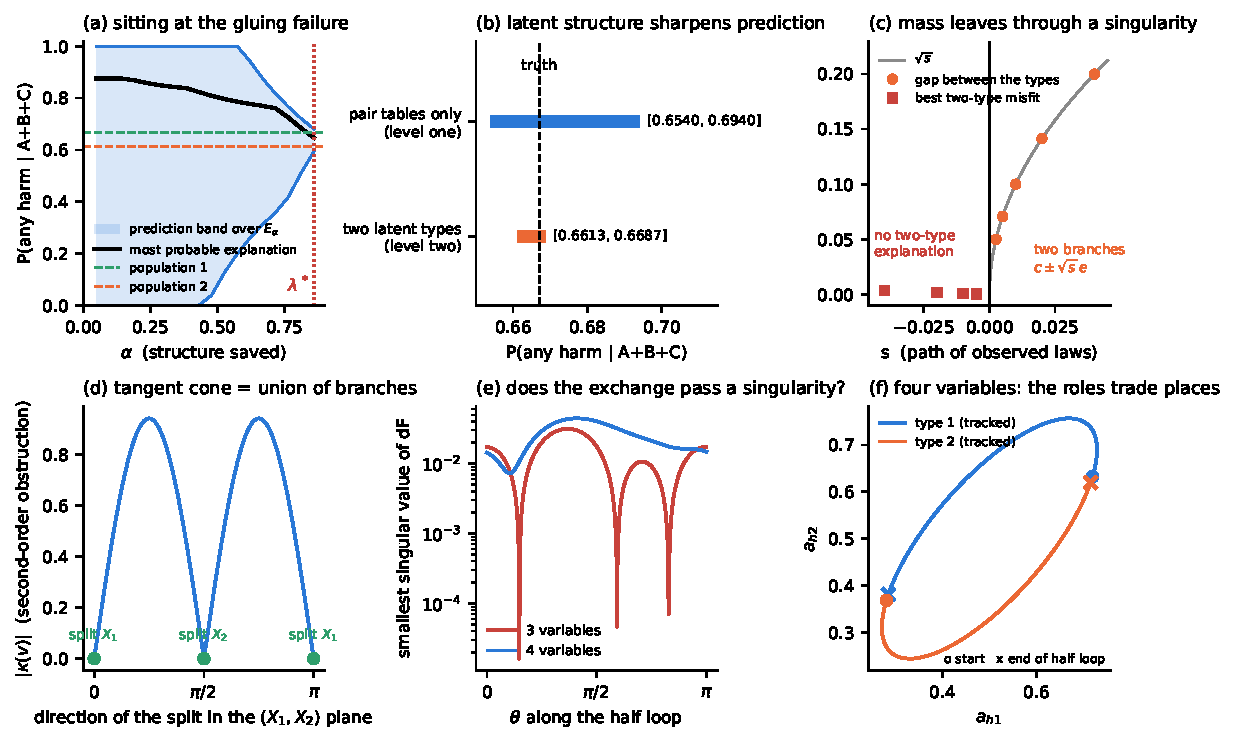
\includegraphics[width=\linewidth]{fig_level2.pdf}
\caption{(a) Graded explanations for the conflicting trials: the prediction band over $E_\alpha$, the most probable explanation, and
the two populations' truths. (b) Level one against two latent types (population~1). (c) Crossing the independence locus: the gap
between the types follows $\sqrt s$; for $s<0$ no two-type explanation fits. (d) The second-order obstruction around the circle of
splits at a coincidence: zero exactly on the coordinate branches. (e) Smallest singular value of $dF$ along a role-exchanging half loop:
with three variables it dips to zero three times, with four it stays away from zero. (f) The 4-variable half loop: the tracked types
trade places.}\label{fig:main}
\end{figure}

\section{Scheme structure: the fibre over independence and the flattening stratification}\label{sec:scheme}

So far ``scheme'' has named the equations of the fibre. This section uses the scheme structure: ideals, their decompositions, reducedness
and flatness. All statements here are checked exactly by Gr\"obner-basis computations \cite{CoxLittleOShea2015} in SymPy \cite{SymPy2017} (\texttt{engine/check\_scheme.py}, SC1--SC6).

\paragraph{Coordinates.}
Replace the susceptibilities by the mean and the difference of the two types,
\[
  \mu=w_1a_1+w_2a_2,\qquad d=a_1-a_2,\qquad\text{so}\qquad a_1=\mu+w_2d,\quad a_2=\mu-w_1d ,
\]
a polynomial automorphism of the parameter space (given $w$). On the observed side use the mean $\mu$ and the central moments
$m_S=E\prod_{i\in S}(X_i-\mu_i)$, $|S|\ge2$: the law and $(\mu,m)$ determine each other polynomially (unitriangularly).

\begin{proposition}[moment normal form; SC1]\label{prop:normal}
$m_S=c_{|S|}(w)\,d_S$ with $d_S=\prod_{i\in S}d_i$ and $c_k(w)=w_1w_2^{\,k}+w_2(-w_1)^k=w_1w_2\big(w_2^{\,k-1}-(-w_1)^{k-1}\big)$.
\end{proposition}

\begin{proof}
$a_{1i}-\mu_i=w_2d_i$ and $a_{2i}-\mu_i=-w_1d_i$, so $m_S=w_1(w_2)^{|S|}d_S+w_2(-w_1)^{|S|}d_S$.
\end{proof}

For fixed weights the map $d\mapsto(c_{|S|}d_S)_S$ is monomial: the two-type model is a toric family over the line of weights. These are
the \emph{secant cumulants} of Michałek, Oeding and Zwiernik \cite{MichalekOedingZwiernik2015}, in which the secant variety becomes
toric. Note $c_2=w_1w_2$ and $c_3=w_1w_2(w_2-w_1)$: an evenly mixed pair leaves no three-way moment.

\paragraph{The fibre over an independent law.}
Let $P=\Pi(c)$ be a product law (the variables independent). Its fibre is where the actors have merged, or one has gone.

\begin{theorem}[the fibre is a Stanley--Reisner scheme; SC2]\label{thm:sr}
The ideal of the fibre over $\Pi(c)$ is
\[
  I=(\mu-c)\;+\;\big(w_1w_2\,d_id_j:\ i<j\big)\;=\;(\mu-c)+\Big[(w_1)\cap(w_2)\cap\bigcap_{i=1}^m(d_j:\ j\neq i)\Big].
\]
It is an intersection of prime ideals, hence radical: the fibre scheme is reduced. With $\mu=c$ it is the Stanley--Reisner scheme
(cut by $w_1+w_2=1$) of the simplicial complex $\Delta$ on the vertices $\{w_1,w_2,d_1,\dots,d_m\}$ with facets
\[
  \{w_1,d_1,\dots,d_m\},\qquad\{w_2,d_1,\dots,d_m\},\qquad\{w_1,w_2,d_i\}\ (i=1,\dots,m).
\]
\end{theorem}

\begin{proof}
By \cref{prop:normal} the fibre is $\mu=c$ and $c_{|S|}(w)d_S=0$ for all $|S|\ge2$. Every $c_k$ is divisible by $c_2=w_1w_2$ and every
$d_S$ with $|S|\ge3$ by some $d_id_j$, so the ideal is $(\mu-c)+(w_1w_2d_id_j)$. Since $w_1$ and $w_2=1-w_1$ are coprime,
$(w_1w_2)=(w_1)\cap(w_2)$; the ideal $(d_id_j:i<j)$ is the Stanley--Reisner ideal of $m$ isolated points, $\bigcap_i(d_j:j\neq i)$; and
the two involve disjoint variables, so their intersection is their product. The facets are the complements of the minimal non-faces
$\{w_1,w_2,d_i,d_j\}$ in the sense of Stanley--Reisner theory \cite{MillerSturmfels2005}. The computation was also checked directly
(Gr\"obner bases for $m=3,4$, and the intersection by elimination).
\end{proof}

The facets are the strata of \cref{tab:strata} named combinatorially: $\{w_1,d_1,\dots,d_m\}$ is ``actor~2 absent, actor~1's
difference free'', $\{w_2,\dots\}$ the reverse, and $\{w_1,w_2,d_i\}$ ``both present, differing only in variable~$i$''. Away from
$w_1w_2=0$ the factor $w_1w_2$ is a unit, so near an interior coincidence the fibre is \emph{exactly} the Stanley--Reisner scheme of $m$
points times the weight line. This upgrades \cref{thm:cone} from the tangent cone to the fibre itself, and since the scheme is reduced
there are no nilpotent directions that the second-order test $\kappa$ could have missed. The simplicial complexes of the gluability
filtration in the companion report \cite{Main} and the singular fibres of level two are therefore the same kind of object.

\paragraph{Three variables: closed form, flatness and the hyperdeterminant.}
For $m=3$ the map $(w_1,\mu,d)\mapsto(\mu,m_{12},m_{13},m_{23},m_{123})$ goes between spaces of dimension 7 and can be inverted. Put
$\Delta_m=m_{12}m_{13}m_{23}$ and $\mathrm{Det}=m_{123}^2+4\Delta_m$.

\begin{proposition}[SC3, SC4]\label{prop:inverse}
\begin{enumerate}[label=(\roman*),leftmargin=*,itemsep=1pt]
\item With $\{i,j,k\}=\{1,2,3\}$, \[w_1w_2=\frac{\Delta_m}{\mathrm{Det}},\qquad w_2-w_1=\pm\sqrt{1-\frac{4\Delta_m}{\mathrm{Det}}},\qquad d_i=\frac{m_{123}}{(w_2-w_1)\,m_{jk}};\] the sign of the square root is the labelling.
\item The Jacobian determinant is $-(w_1w_2)^3(d_1d_2d_3)^2$.
\item $\mathrm{Det}$ is Cayley's hyperdeterminant \cite{GelfandKapranovZelevinsky1994} of the $2\times2\times2$ table of the law.
\end{enumerate}
\end{proposition}

\begin{theorem}[flattening stratification, $m=3$; SC5]\label{thm:flat}
Over the space of laws:
\begin{center}\small
\begin{tabular}{lll}\toprule
laws & fibre & flat\\\midrule
all $m_{ij}\neq0$, $\mathrm{Det}\neq0$ & two reduced points (labels swap) & yes (\'etale, degree 2)\\
one variable independent of the other two & a surface & no\\
product laws & Stanley--Reisner scheme (dim.~3) & no\\
exactly one $m_{ij}=0$; or $\mathrm{Det}=0\neq\Delta_m$ & empty (closure only) & ---\\\bottomrule
\end{tabular}
\end{center}
On the parameter side the map is flat exactly off $\{w_1w_2d_1d_2d_3=0\}$: where an actor is absent or the actors agree on a variable.
On the generic stratum the real points are: two genuine mixtures ($w\in(0,1)$) if $\Delta_m>0$; two signed mixtures (real, but
$w\notin[0,1]$) if $\mathrm{Det}>0>\Delta_m$; a complex-conjugate pair if $\mathrm{Det}<0$.
\end{theorem}

\begin{proof}
The fibres are read off \cref{prop:inverse} and checked by Gr\"obner bases. Flatness: source and target are regular of the same dimension,
so by ``miracle flatness'' \cite[Thm.~23.1]{Matsumura1986} the map is flat at a point iff the fibre through it has dimension $0$ there;
the Jacobian vanishes exactly on $w_1w_2d_1d_2d_3=0$, and those points lie in the positive-dimensional fibres of the second and third rows.
Real points: $p=w_1w_2=\Delta_m/\mathrm{Det}$ is real and $1-4p=m_{123}^2/\mathrm{Det}$. If $m_{123}\neq0$, $w$ is real iff
$\mathrm{Det}>0$, and then $d$ is real by (i). If $m_{123}=0$, then $w=(\frac12,\frac12)$ and $d_i^2=m_{ij}m_{ik}/(p\,m_{jk})$ has the sign of
$\Delta_m$, which here is the sign of $\mathrm{Det}=4\Delta_m$. In both cases $w\in(0,1)$ iff $p\in(0,\frac14]$ iff $\Delta_m>0$. The sign of $\mathrm{Det}$ separates real tensor rank 2
from 3, as in de~Silva and Lim \cite{deSilvaLim2008}.
\end{proof}

This corrects the picture of \cref{sec:puiseux}. The fold where real explanations disappear is \emph{not} where flatness fails: over
$\mathbb C$ the two explanations persist and become conjugate. What the stratification gives is the following.

\begin{corollary}[where explanations can die]\label{cor:die}
Along a continuous path of laws, a two-type probability explanation (parameters in the box $w\in[0,1]$, $a\in[0,1]^{2m}$, $m=3$) can cease
to exist only (a) by reaching a wall of the box, or (b) at a law where its limit lies in the non-flat locus $\{w_1w_2d_1d_2d_3=0\}$.
\end{corollary}

\begin{proof}
On $\{\Delta_m>0\}$ the inverse is continuous (\cref{prop:inverse}, $\mathrm{Det}\ge4\Delta_m>0$), so an explanation persists while the
path stays there and inside the box. If the path leaves $\{\Delta_m>0\}$ at a law $P^*$ while the explanations stay in the compact box, a
limit point $x^*$ has $F(x^*)=P^*$ with $\Delta_m(P^*)=(w_1w_2)^3(d_1d_2d_3)^2=0$.
\end{proof}

The box wall is the semialgebraic part, invisible to the scheme; the inequalities that cut the probability image out of the secant variety
are those of Allman, Rhodes, Sturmfels and Zwiernik \cite{AllmanRhodesSturmfelsZwiernik2015} (see also \cite{Zwiernik2016}).

\begin{corollary}[monodromy from the stratification]\label{cor:mono}
Over $\{\Delta_m>0\}$ the sign of $d_1$ is a continuous, nowhere-zero label of the two sheets, so the real double cover of genuine mixtures
is trivial: roles cannot be exchanged without leaving through the non-flat locus (\cref{thm:m3}). Over $\mathbb C$ the cover is connected and
its monodromy is $\mathbb Z/2$. For $m=4$, a variable independent of the rest ($d_4=0$) is a flat point (full rank, two points; SC6), the
non-flat walls move to codimension $\ge2$ and no longer separate the real region, which is why the 4-variable loop of
\cref{sec:monodromy} can exchange roles.
\end{corollary}

We expect that for every $m\ge3$ the map is flat exactly where $w_1w_2\neq0$ and at least three $d_i$ are non-zero (consistent with
\cite{AllmanMatiasRhodes2009}); we have checked this only for $m=3$ and at a point for $m=4$.

\paragraph{The image.}
The Zariski closure of the image of the $k$-type model is the $k$-th secant variety of the Segre embedding of $(\mathbb P^1)^m$ \cite{Landsberg2012}. For $k=2$,
$m=3$ it fills $\mathbb P^7$ (generic $2\times2\times2$ tensors have rank 2), which is why the boundary of the two-type region is real and
semialgebraic (the walls $\Delta_m=0$, $\mathrm{Det}=0$ and the box), not Zariski-closed. For $m\ge4$ the secant variety has dimension
$2m+1<2^m-1$ and is a proper subvariety, toric in secant cumulants \cite{MichalekOedingZwiernik2015}. \Cref{fig:scheme} shows the three real
regions on a slice, the complex $\Delta$, and a path crossing the walls.

\begin{figure}[!htbp]\centering
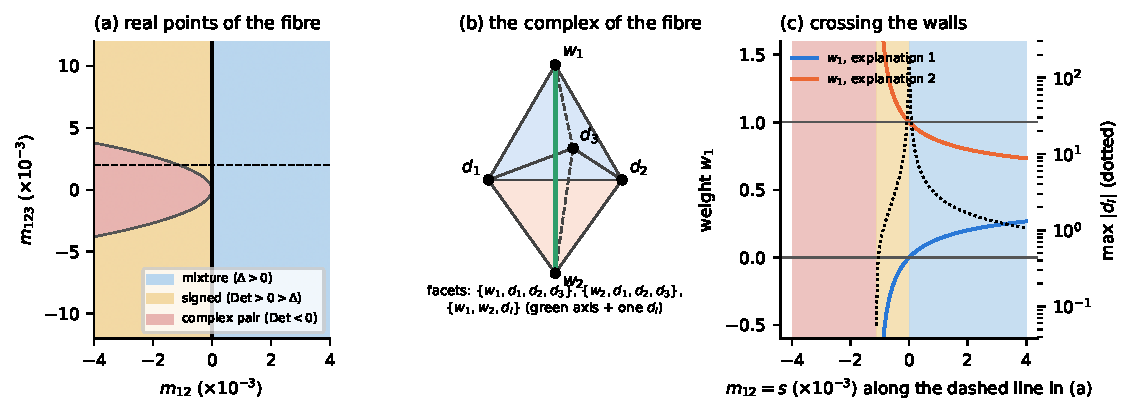
\includegraphics[width=\linewidth]{fig_scheme.pdf}
\caption{(a) A slice of the law space ($m_{13}=m_{23}=0.03$, mean fixed) coloured by the real points of the two-type fibre: genuine
mixtures ($\Delta_m>0$), signed mixtures ($\mathrm{Det}>0>\Delta_m$), complex-conjugate pairs ($\mathrm{Det}<0$, inside the parabola
$m_{123}^2=-4\Delta_m$). (b) The simplicial complex $\Delta$ of \cref{thm:sr} for $m=3$: two tetrahedra on the triangle $d_1d_2d_3$, and
the axis $w_1w_2$ with the triangles $\{w_1,w_2,d_i\}$; its Stanley--Reisner scheme is the fibre over an independent law. (c) Along the
dashed line of (a): the weights of the two explanations (they leave $[0,1]$ as the path crosses $m_{12}=0$, where one weight tends to $0$
and $\max|d_i|$ blows up, and they are complex beyond $\mathrm{Det}=0$). A probability explanation also needs $|d_i|\le1$, so in practice it
hits the box wall before $m_{12}=0$.}\label{fig:scheme}
\end{figure}

\section{The ladder of base semirings}\label{sec:ladder}

The two levels fail in the same way: their equations have points over a larger number system but not over the non-negative one. We make
this a single picture. Write the evidence at either level as polynomial equations with rational coefficients, and present a probability
$a$ together with its complement $\bar a=1-a$, so that the parameter box is cut out by $a,\bar a\ge0$. Then ask over which semiring the
equations have points:
\[
  \mathbb C\ \supset\ \R\ \supset\ \R_{\ge0}.
\]
An $\R_{\ge0}$-point is a probability explanation; an $\R$-point that is not one is a signed explanation (a quasi-probability, or actors
with negative weight); a $\mathbb C$-point that is not real is an oscillatory explanation; and no point at all is the bottom of the
ladder. Each rung has its own measure of how badly the next rung up fails (\cref{tab:ladder}).

\begin{table}[!htbp]\centering\small
\begin{tabular}{p{0.11\linewidth}p{0.4\linewidth}p{0.4\linewidth}}\toprule
rung & level one (a law on outcomes) & level two (two latent actors, three variables)\\\midrule
none & the tables disagree on an overlap (signalling, a direct influence); measured by the \emph{linear gap}, the least $\ell_1$ repair & not in the image: one pairwise moment zero alone, or $\mathrm{Det}=0\neq\Delta_m$\\
$\mathbb C$ & same as $\R$ (linear equations) & $\mathrm{Det}<0$: a complex-conjugate pair; measured by the imaginary part\\
$\R$ & contextual: a signed global section exists, no positive one; measured by the \emph{negativity} $\nu$ & signed mixture, $\mathrm{Det}>0>\Delta_m$; measured by the negative weight $\nu_2=\tfrac12\big(|m_{123}|/\sqrt{\mathrm{Det}}-1\big)$\\
$\R_{\ge0}$ & the tables glue ($\lambda^*=1$) & genuine mixture, $\Delta_m>0$; then the box $a\in[0,1]$ is a further semialgebraic wall\\\bottomrule
\end{tabular}
\caption{The ladder at both levels. Level one has no complex rung, because its equations are linear; level two has one, because they
are not.}\label{tab:ladder}
\end{table}

\paragraph{Level one.}
Let $A\mu=t$ be the marginal equations of a family of windows, with $\mu$ a signed measure of total mass $1$. The \emph{linear gap} is
$\min\|A\mu-t\|_1$, and when it is zero the \emph{negativity} is $\nu=\min\{\|\mu^-\|:A\mu=t\}$, the least total negative mass of a signed
global section; both are linear programs. The negativity is the quantity behind Abramsky and Brandenburger's operational reading of
negative probabilities \cite{AbramskyBrandenburger2014}.

\begin{theorem}[the ladder at level one; LD1--LD3]\label{thm:ladder1}
\begin{enumerate}[label=(\roman*),leftmargin=*,itemsep=1pt]
\item $\mathbb C$-points exist iff $\R$-points exist iff the linear gap is $0$; for the measurement scenarios we test (cycles, CHSH,
three outcomes) this holds whenever the tables agree on their overlaps \cite{AbramskyBrandenburger2011}.
\item $\R_{\ge0}$-points exist iff $\nu=0$ iff $\lambda^*=1$.
\item On the set of families with linear gap $0$ (a polytope), $\nu$ and $1-\lambda^*$ are comparable: there are constants $0<c_-\le c_+$
depending only on the scenario with $c_-(1-\lambda^*)\le\nu\le c_+(1-\lambda^*)$. One can take $c_+=\nu(r)$ maximised over the
no-signalling polytope.
\end{enumerate}
\end{theorem}

\begin{proof}
(i) The equations are linear with rational coefficients, so solvability over $\mathbb C$, $\R$ and $\mathbb Q$ coincide; the gap is the
$\ell_1$ distance to solvability. (ii) A signed section with $\nu=0$ is a global law, and conversely. (iii) Upper bound: write $t_w=\lambda^*q|_w+
(1-\lambda^*)r_w$ as in \eqref{eq:split}. The residues $r_w$ agree on overlaps because $t$ and $q|_w$ do, so $r$ has a signed section
$\mu_r$, and $\lambda^*q+(1-\lambda^*)\mu_r$ is a signed section of $t$ with negativity $(1-\lambda^*)\nu(\mu_r)$. Lower bound: $\nu$ and
$1-\lambda^*$ are both convex and piecewise linear in $t$ (values of linear programs with $t$ in the right-hand side), and they vanish on
the same polytope, the noncontextual polytope. A polyhedral convex function grows at least linearly away from its zero set (weak sharp
minima \cite{BurkeFerris1993}, a form of Hoffman's bound \cite{Hoffman1952}), and the other is Lipschitz and vanishes there; so each is
bounded by a multiple of the distance to that polytope, and hence by a multiple of the other.
\end{proof}

The constants depend on the scenario, and we measured them (\cref{fig:ladder}(a), 30 random mixtures of a global law with a contextual
family in each of five scenarios). The ratio $\nu/(1-\lambda^*)$ is exactly $\tfrac12$ for the 3-cycle, the 4-cycle and CHSH \cite{CHSH1969} with the
Popescu--Rohrlich box \cite{PopescuRohrlich1994}, exactly $\tfrac14$ for the anti-correlated 5-cycle, and between $\tfrac12$ and $\tfrac23$ for a three-outcome
triangle, never exceeding the contextual part's own negativity. So the negativity is not a fixed multiple of the unsavable fraction; the
two measure the same thing, but in different units.

The drug example sits on the bottom rung. In \cref{ex:conflict} the $B$ margin differs between the two populations ($P(H_B)$ is $0.26$ in
one and $0.40$ in the other), so the pair tables disagree on an overlap: there is no signed global law at all, and the linear gap is
$0.28$. Yet $\lambda^*=0.86$: the graded explanations of \cref{sec:graded} are about sub-measures, and they still save $86\%$ of the
structure. In the language of contextuality-by-default \cite{DzhafarovKujala2016} this is a direct influence, not contextuality; the
ladder separates the two, and $\lambda^*$ measures both together. Population~1 alone is on the top rung.

\paragraph{Level two.}
For two actors and three variables, \cref{thm:flat} already places every generic law on a rung. The measures follow from
\cref{prop:inverse}: since $1-4w_1w_2=m_{123}^2/\mathrm{Det}$, the weights are $\tfrac12(1\pm|m_{123}|/\sqrt{\mathrm{Det}})$, so on the
$\R$ rung the negative weight is $\nu_2=\tfrac12(|m_{123}|/\sqrt{\mathrm{Det}}-1)$, which tends to $0$ as $\Delta_m\to0^-$ and to
$\infty$ as $\mathrm{Det}\to0^+$. On the $\mathbb C$ rung the imaginary parts measure the failure; along the Puiseux path of
\cref{sec:puiseux} the explanation for $s<0$ is $c\pm i\sqrt{|s|}\,e$, with imaginary part $2\sqrt{|s|}\max_i|e_i|$ in $d$.

\begin{proposition}[how a law moves between rungs; LD4--LD6]\label{prop:moves}
For $m=3$ a two-type explanation moves between rungs only (a) across $\mathrm{Det}=0$, where the weights diverge, (b) across $\Delta_m=0$,
either through a non-flat stratum or through a point of the closure that is not in the image, where one weight passes through $0$ while
$\max|d_i|$ diverges, or (c) across a wall of the box. In (a) and in the second case of (b) the fibre has a point at infinity: the
map is not proper there.
\end{proposition}

\begin{proof}
The rung is determined by the signs of $\mathrm{Det}$ and $\Delta_m$ and by the box (\cref{thm:flat}). By \cref{prop:inverse}, $w_1w_2=
\Delta_m/\mathrm{Det}$ diverges as $\mathrm{Det}\to0$ with $\Delta_m\neq0$; and $\Delta_m\to0$ with $\mathrm{Det}\to m_{123}^2\neq0$ sends one
weight to $0$ and, if only one pairwise moment vanishes, $d_k=m_{123}/((w_2-w_1)m_{ij})$ to infinity.
\end{proof}

The checks confirm the closed-form rung against how each law was made (200 genuine mixtures, 200 valid laws made from signed weights, and
complex cases confirmed by an exact Gr\"obner solve; about $8\%$ of laws drawn at random from a Dirichlet distribution lie on the complex
rung), and follow a path across all the walls (\cref{fig:ladder}(b)).

\begin{figure}[!htbp]\centering
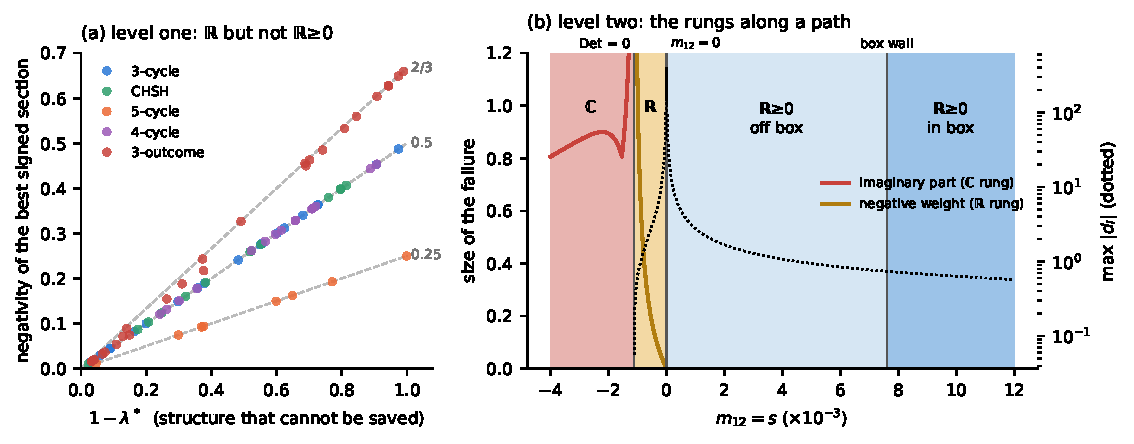
\includegraphics[width=\linewidth]{fig_ladder.pdf}
\caption{(a) Level one: the negativity of the best signed global section against $1-\lambda^*$ for no-signalling families in five
scenarios; each lies on or between lines whose slope is its contextual part's own negativity. (b) Level two, along the path $m_{12}=s$
($m_{13}=m_{23}=0.03$, $m_{123}=0.002$, means $\tfrac12$): the rung of the two-type explanation, the imaginary part on the $\mathbb C$ rung,
the negative weight on the $\R$ rung, and $\max|d_i|$ (dotted), which diverges at $m_{12}=0$. The explanation enters the box at
$s\approx0.0076$.}\label{fig:ladder}
\end{figure}

\paragraph{What the ladder says.}
Incoherence comes in kinds, and the kinds are the rungs. Disagreement on an overlap is the bottom rung: no number system rescues it, and
the only remedy is to move the evidence (the consistency radius, the linear gap). Contextuality is the $\R$ rung at level one: the
evidence is consistent as linear algebra but needs negative probability. At level two the same rung means actors with negative weight,
and a new rung appears below it: actors that exist only as complex conjugates. The gradation of \cref{sec:graded} cuts across the ladder,
since $\lambda^*$ (or $\lambda^*_2$) measures how much of the evidence can be saved on the top rung whatever rung the whole sits on. The
scheme fixes the equations; the semiring decides whether their points are probabilities. A single semiring scheme carrying both levels, with
$\lambda^*$ read from it, is the step this section motivates but does not take.

\section{Obstructions to commutativity as structure}\label{sec:noncomm}

Everything so far is commutative: probabilities are numbers, and the order in which evidence is taken does not matter. Here we let the
coefficients be matrices. A state is a density matrix $\rho$ (Hermitian, positive semidefinite, trace $1$), an observable is a projective
measurement $\{A_a\}$ (orthogonal projections summing to the identity), and spatial arrangement enters through rotations: the spin-$j$
component $n\cdot J$ along a direction $n$. The aim is not to discard what fails to commute but to give it a place. It finds three:
the cover of contexts, the complex rung of the ladder, and the holonomy of loops. All statements are checked in
\texttt{engine/check\_noncomm.py} (NC1--NC8).

\paragraph{Commutators decide the cover.}
Observables that commute can be measured together. The contexts are therefore the maximal sets of pairwise commuting observables (cliques
of the commutation graph), and a state $\rho$ assigns each context its joint table $\mathrm{tr}(\rho\prod_iA^{(i)}_{a_i})$. These tables agree on
overlaps automatically. If all observables commute there is one context and the tables glue (the joint spectral measure; NC1). Gluing can
fail only through non-commutativity. For the CHSH observables the commutation graph has exactly the four Bell contexts, and at
Tsirelson's angles \cite{Tsirelson1980} the engine's noncontextual fraction is $\lambda^*=2-\sqrt2$, the known value. As the angle
between $A_0$ and $A_1$ opens from $0$, $\|[A_0,A_1]\|$ grows from $0$ and $\lambda^*$ falls from $1$ (NC3, \cref{fig:noncomm}(b)). Classically the
cover was given; here it is derived from the algebra, and the gluing questions of \cref{sec:graded,sec:ladder} sit on top of it.

\paragraph{Order is bounded by the commutator.}
Measuring $P$ then $Q$ (Lüders' rule \cite{Luders1951}) gives $\mathrm{tr}(QP\rho PQ)$, so the order effect is
$O=\mathrm{tr}\big(\rho\,(PQP-QPQ)\big)$.

\begin{proposition}[NC2]\label{prop:order}
$|O|\le\|[P,Q]\|$ for every state, and the QQ equality $p(P,\bar Q)+p(\bar P,Q)=p(Q,\bar P)+p(\bar Q,P)$ holds for every pair of binary
projective measurements.
\end{proposition}

\begin{proof}
By the two-subspace theorem \cite{Halmos1969} the space splits into blocks where $P$ and $Q$ commute (contributing $0$) and $2\times2$
blocks with an angle $\theta$, where $P=\begin{psmallmatrix}1&0\\0&0\end{psmallmatrix}$ and $Q$ projects onto $(\cos\theta,\sin\theta)$. There
$PQP-QPQ=\cos^2\theta\,(P-Q)$, of norm $\cos^2\theta\,|\sin\theta|\le|\cos\theta\sin\theta|=\|[P,Q]\|$ on the block. The QQ equality follows by
expanding with $\bar P=1-P$, $\bar Q=1-Q$: $P\bar QP+\bar PQ\bar P=P+Q-PQ-QP$, which is symmetric in $P$ and $Q$, so both sides equal
$\mathrm{tr}\big(\rho(P+Q-PQ-QP)\big)$.
\end{proof}

The QQ equality is the test Wang, Solloway, Shiffrin and Busemeyer applied to order effects in survey questions
\cite{WangBusemeyer2014}; it holds for any projective model and constrains the order effects that commutation leaves.

\paragraph{The canonical section lives on the complex rung.}
For two measurements $A$ and $B$ the Kirkwood--Dirac table \cite{Kirkwood1933,Dirac1945,ArvidssonShukur2024}
\[
  q(a,b)=\mathrm{tr}(B_bA_a\rho)
\]
has exactly the right marginals, $\sum_bq(a,b)=\mathrm{tr}(A_a\rho)$ and $\sum_aq(a,b)=\mathrm{tr}(B_b\rho)$: it is a global section of the two
tables. But its entries are complex, and
\[
  \mathrm{Im}\,q(a,b)=\tfrac1{2i}\,\mathrm{tr}\big([B_b,A_a]\rho\big),
\]
so the imaginary part is an expectation of commutators (NC4). If $A$ and $B$ commute, $B_bA_a$ is a projection and $q$ is a law: the top
rung. Real projections with a real state give a real $q$ that can be negative: the $\R$ rung. Otherwise $q$ is non-real: the $\mathbb C$
rung. At level one, with numbers as coefficients, the complex rung was empty (\cref{tab:ladder}); with matrices it is inhabited, and its
inhabitants are exactly the commutation obstructions. This is a finer statement than $\lambda^*$. Two contexts that do not overlap
always glue classically (take the product), so $\lambda^*=1$ there; what fails is that the section the state itself determines is not a
law. Pusey showed that anomalous weak values, which are ratios of Kirkwood--Dirac entries, are proofs of contextuality
\cite{Pusey2014}.

\paragraph{Loops leave a phase, and the phase can be non-abelian.}
Around a loop of rank-one projections the product $\mathrm{tr}(P_1P_2P_3)$ (the Bargmann invariant \cite{Bargmann1964}) is gauge-invariant.
For spin $\tfrac12$ its argument is half the signed solid angle of the spherical triangle, the Pancharatnam--Berry phase
\cite{Pancharatnam1956,Berry1984}; for real projections it is real (NC5, \cref{fig:noncomm}(d)). Complex coefficients are therefore
what makes loops carry information: the phase is invisible in each probability and appears only in the order of the product. For
spin $j$, densely sampled loops return the state with phase $j\Omega$ (NC8), so two paths to the same target with the same success
probability differ by a geometric phase. With rank-two projections the loop acts on the subspace by a $2\times2$ unitary, and two
different loops give unitaries that do not commute (NC6): the holonomy is non-abelian \cite{WilczekZee1984}. This is where the
$\mathbb Z/2$ exchange of actors in \cref{sec:monodromy} goes once actors carry matrices: the discrete swap becomes one element of a
continuous, non-abelian holonomy.

\paragraph{Probability paths.}
Projections that do not commute can steer. Start in $|j,j\rangle$ along $n_0$ and measure $n\cdot J$ along $N$ equally spaced directions on
the great circle to $n_1$ (angle $\Theta$). Each step keeps the tracked outcome with probability $|d^{\,j}_{jj}(\Theta/N)|^2=
\cos^{4j}(\Theta/2N)$, so
\[
  P_N=\cos^{4jN}\!\Big(\frac{\Theta}{2N}\Big)\ \longrightarrow\ 1\qquad(N\to\infty),
\]
against $\cos^{4j}(\Theta/2)$ for the direct jump (NC7, exact for $j=\tfrac12,1,\tfrac32$; \cref{fig:noncomm}(c)). This is Zeno dragging
\cite{MisraSudarshan1977,AharonovVardi1980}. Projections that commute with each other and with the state can only condition; they never
move it (NC7). Read as an analogy for molecular arrangements: a configuration that is improbable in one step can be reached with probability
close to one along a path of intermediate arrangements, the route matters through the geometric phase even when the success probability
does not, and the whole effect lives in the non-commutativity. Whether a given chemical system behaves this way is a physical question
these toy spin models do not answer.

\begin{figure}[!htbp]\centering
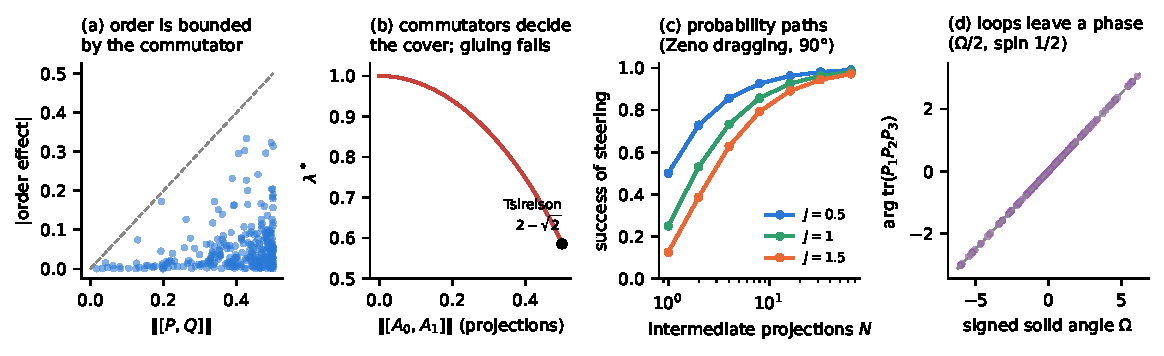
\includegraphics[width=\linewidth]{fig_noncomm.pdf}
\caption{(a) Order effects against $\|[P,Q]\|$ for 300 random pairs of projections: all below the diagonal (\cref{prop:order}).
(b) The CHSH family: as the angle between $A_0$ and $A_1$ opens, the commutator grows and $\lambda^*$ falls from $1$ to $2-\sqrt2$.
(c) Zeno dragging through $90^\circ$: success against the number of intermediate projections, for spin $j=\tfrac12,1,\tfrac32$.
(d) The loop phase $\arg\mathrm{tr}(P_1P_2P_3)$ against the signed solid angle for 200 random spin-$\tfrac12$ triangles: the line
$\Omega/2$.}\label{fig:noncomm}
\end{figure}

\paragraph{What survives of the scheme picture.}
For a fixed matrix dimension $d$, take the real and imaginary parts of the entries as coordinates: marginals (partial traces) are linear,
Born probabilities quadratic, and $\rho\succeq0$ a set of polynomial inequalities. Explanations are again real points of a commutative
scheme, and the strata become rank conditions. Three things change. The positive cone is the positive semidefinite cone, which is not a
semiring, so the ladder of \cref{sec:ladder} becomes a ladder of cones, classical $\subset$ quantum $\subset$ signed (between local and
no-signalling sits the quantum set, approximated by the NPA hierarchy \cite{NPA2007}). Actors carrying matrices have a unitary gauge
freedom, so fibres become orbits and the right object is the quotient, whose coordinate ring is generated by trace polynomials
\cite{Procesi1976}. And if $d$ is not fixed there is no single scheme: the observables generate a non-commutative algebra whose
representation schemes $\mathrm{Rep}_d$ form a tower \cite{LeBruyn2008}. Whether some $d$ explains the data is the question behind Tsirelson's
problem, and it is undecidable in general \cite{Slofstra2019,MIPRE2020}. Our classical results are the diagonal sector of this picture.
Whether the fibre over a merge point stays reduced once off-diagonal (coherence) directions are allowed is the first open scheme-theoretic
question here.

\section{Given measurements, partly masked}\label{sec:masked}

\Cref{sec:noncomm} ended at a fork: either the measurements are given, or they too are unknown, in which case deciding whether some
dimension explains the data is undecidable in general. Here we take the measurements as given and then hide a fraction of them, to see how
the difficulty grows and how much geometry and positivity still recover. At a fixed dimension nothing becomes undecidable: the questions
are first-order statements over the reals and so decidable by quantifier elimination \cite{BasuPollackRoy2006}. What grows is the cost,
the non-convexity, and the size of the set of explanations. All results are in \texttt{engine/check\_masked.py} (MK1--MK6) and
\texttt{engine/check\_masked\_gauge.py} (MK7).

\paragraph{Setting.}
Two qubits; Alice measures spin along $K=5$ known directions $a_i$, Bob along $K=5$ known directions $b_j$; every pair is a context whose
$2\times2$ table is observed with $N=2000$ shots, from a random entangled state mixed with $15\%$ noise. A masked direction still has its
tables observed, but the solver does not know it. With Bloch vectors $s,t$ and correlation matrix $T$,
\[
  P(\alpha,\beta\mid a,b)=\tfrac14\big(1+\alpha\,s\cdot a+\beta\,t\cdot b+\alpha\beta\,a^{\!\top}Tb\big),
\]
linear in the state for fixed directions and linear in each direction for a fixed state. With nothing masked the state is a linear
least-squares fit, unique and positive within noise (MK1).

\paragraph{What the linear fit can see.}
\begin{proposition}[MK5, MK7]\label{prop:linmask}
Let Alice's known directions span $V\subseteq\R^3$ and let $h_A$ of her directions be masked; let Bob's directions span $\R^3$. Then the
tables do not change if each hidden direction $n$ is replaced by $Mn$ and the state by $s\mapsto M^{-\top}s$, $T\mapsto M^{-\top}T$, for any
$M\in GL_3$ that fixes $V$ pointwise. The linear fit therefore leaves the hidden directions ambiguous along this group, cut by unit length:
a family of dimension $\max\big(0,\,3(3-\dim V)-h_A\big)$. In particular the hidden directions are located by the linear fit iff the known
directions on their side span $\R^3$; and with three directions per side and $\dim V=2$, the fit is the same for every candidate direction.
\end{proposition}

\begin{proof}
Alice's data enter only through $s\cdot a$ and $a^{\!\top}Tb$. For a known $a\in V$, $(M^{-\top}s)\cdot a=s\cdot M^{-1}a=s\cdot a$ and likewise for
$T$; for a hidden $n$, $(M^{-\top}s)\cdot Mn=s\cdot n$. The group of $M$ fixing $V$ pointwise has dimension $3(3-\dim V)$, and unit length
imposes one condition per hidden direction. The dimension count is checked as the kernel of the Jacobian at the truth in seven cases
($\dim V=3,2,1$; $h_A=1,2,3$), all equal to the prediction (MK7). With three directions per side the nine tables carry exactly the fifteen
state parameters, so for planar known directions the residual is zero at $92\%$ of lattice points (the rest lie near the plane, where the
three directions become dependent; MK5).
\end{proof}

When the known directions span $\R^3$, the linear fit has one basin: refining from the best lattice point recovers a hidden direction
exactly on noiseless data (\cref{fig:masked}(c)).

\paragraph{What the cone adds: culling impossible points.}
When the linear fit is blind, positivity is not. Every candidate direction implies a fitted state; if that state has a negative
eigenvalue, it assigns negative probability to some measurement, and the candidate is not merely improbable but impossible. On a lattice
this is one eigenvalue per point. In the planar case (two known directions in a plane and one hidden out of it, on each side) only
$0.01\%$ of the $40{,}000$ lattice points imply a positive state; none of them is the truth, because the feasible set is a small region
that a $14^\circ$ lattice misses. Using the smallest eigenvalue as a score, keeping the best lattice points, and climbing from them finds
the feasible set, which contains the truth, is closed under the mirror (global complex conjugation, which preserves positivity), and
bounds invariants: over $1434$ feasible samples the CHSH maximum \cite{Horodecki1995} lies in $[2.254,2.452]$ (truth $2.354$), and a
held-out correlation in $[0.159,0.256]$ (truth $0.211$) (MK6, \cref{fig:masked}(d)). A mirror applied to one side only is a partial
transpose, which does not preserve positivity for entangled states \cite{Peres1996}, so the cone removes one-sided ambiguities while
keeping the two-sided one.

\paragraph{Random masking.}
\Cref{tab:masked} summarises six random trials at each level (fresh state and directions each time). Hiding one or two of ten directions
always leaves at least three known on each side, so the linear fit locates them: an exhaustive lattice of $300$ directions per hidden
direction is culled to under $2\%$ by the fit alone, and in every trial whose known directions are well-conditioned ($9$ of $12$) exactly one
explanation survives the cone (MK2). The exception is instructive. In one trial at $20\%$, with nearly coplanar known directions, the linear
fit left three explanations and none of them implies a positive state, although the truth lies inside the $\chi^2$ set: when the geometry
is nearly degenerate the positive explanation sits away from the linear optima, and positivity has to drive the search, as in the planar
case above, rather than be applied afterwards. At $30\%$ and $50\%$ the exhaustive lattice would
need $300^h$ fits, so coordinate-wise lattice sweeps take over; they reach the best explanation found by any method (MK3). The errors are
large exactly in the trials where a side keeps fewer than three independent known directions, as \cref{prop:linmask} predicts.

\begin{table}[!htbp]\centering\small
\begin{tabular}{lccccc}\toprule
masked & located linearly & median error & truth in 99\% set & fits used & local-search success\\\midrule
$0\%$ & 6/6 & $0^\circ$ & 6/6 & 1 & ---\\
$10\%$ (1 of 10) & 6/6 & $3.0^\circ$ & 5/6 & 300 & 0.94\\
$20\%$ (2) & 6/6 & $3.5^\circ$ & 6/6 & 90{,}000 & 0.81\\
$30\%$ (3) & 4/6 & $4.4^\circ$ (others $67^\circ$) & 6/6 & 16{,}200 & 0.74\\
$50\%$ (5) & 0/6 & (all $49^\circ$) & 6/6 & 27{,}000 & 0.69\\\bottomrule
\end{tabular}
\caption{Masked measurements, six trials per level. ``Located linearly'': each side keeps known directions spanning $\R^3$. The error is
the largest angle between a recovered and a true hidden direction. Fits: exhaustive lattice for one and two hidden directions, lattice
sweeps beyond. Local search: the fraction of random starts of plain least squares that reach the best explanation.}\label{tab:masked}
\end{table}

Three further points. The coverage of the $99\%$ $\chi^2$ set was $11$ of $12$ at $10$--$20\%$, so the Gaussian approximation behind it is
somewhat optimistic. The operator-free rungs of \cref{sec:ladder} are computed from the tables alone, so masking does not touch them: the
noncontextual fraction of the tables was between $0.947$ and $0.967$ in the sampled trials, whatever was hidden (MK4). And what can be
extracted is exactly what is invariant under the residual symmetry: the CHSH maximum survives the mirror and is pinned by the cone, while a
correlation with a new direction is not invariant and has a wider interval. In the language of \cref{sec:noncomm}, what masked
measurements leave recoverable are the functions on the quotient by the residual group, cut down by positivity.

\begin{figure}[!htbp]\centering
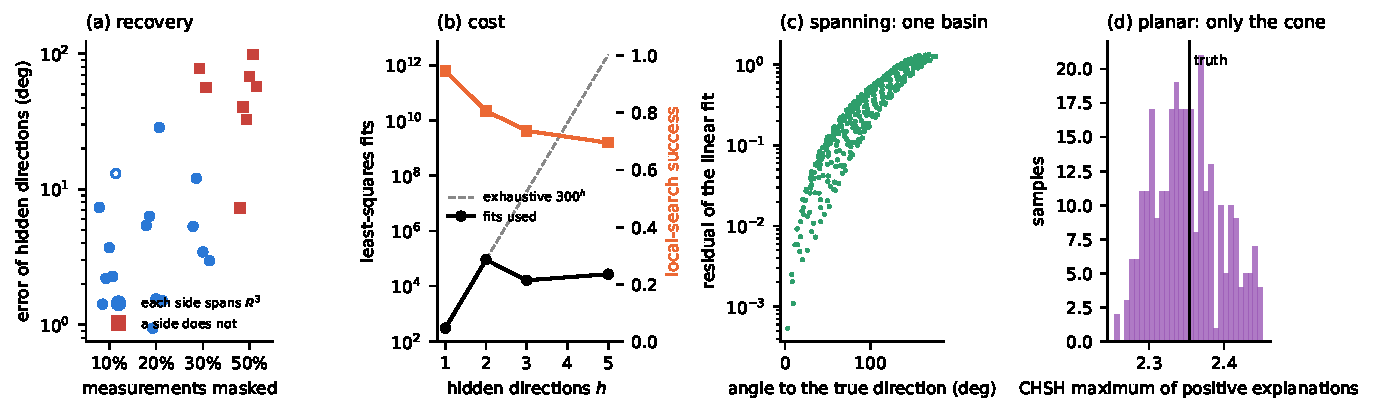
\includegraphics[width=\linewidth]{fig_masked.pdf}
\caption{(a) Error of the recovered hidden directions against the masking level, split by whether each side keeps known directions
spanning $\R^3$ (circles) or not (squares); an open marker is a trial whose truth fell outside the $99\%$ set. (b) Cost: least-squares
fits used (exhaustive lattice up to two hidden directions, sweeps beyond) against the exhaustive count $300^h$, and the success rate of
plain local search. (c) Spanning known directions: the residual of the linear fit over the lattice against the angle to the true
direction: one basin. (d) Planar known directions: the linear fit is blind, the cone is not; the CHSH maximum over the feasible (positive)
explanations against the truth.}\label{fig:masked}
\end{figure}

\section{Quantum graded gluing: positivity domains of hereditary quadratics}\label{sec:qglue}

Islam, Volčič and Woerdeman study self-adjoint matrix polynomials $f=L+H^*H-K^*K$ in non-commuting variables $x_j$ and their adjoints,
evaluated on tuples of matrices of every size, and their positivity domains $\mathcal D(f)$, where $f$ is positive semidefinite
\cite{IVW2026}. Graded gluing with quantum windows is exactly of this form. All statements here are checked in
\texttt{engine/check\_qglue.py} (QG1--QG6).

\paragraph{The identification.}
Let the windows be sets of qubits with density matrices $\rho_w$, and let $\psi$ be an unnormalised global vector. The quantum form of
$\alpha\,q|_w\le t_w$ is
\[
  \mathrm{Tr}_{\mathrm{rest}}(\psi\psi^*)\preceq\rho_w\quad\text{for every window,}\qquad\text{with mass }\alpha=\|\psi\|^2 .
\]
Ordering $\psi$ as $\psi_{ak}$ (window index $a$, the rest $k$) and putting $K=\sum_{a,k}|k\rangle\langle a|\,x_{ak}$, the constraint is
$f_w(\psi)\succeq0$ for $f_w=\rho_w^{\top}-K^*K$, a self-adjoint hereditary quadratic with constant term and no linear term. The family gives
$f=\bigoplus_wf_w$, and the quantum explanations are its positivity domain. The paper's hypotheses hold (QG1): the quadratic coefficients
generate the full matrix algebra (coefficient-irreducible); the line system is minimal; the linearisation
$\begin{psmallmatrix}I&K\\K^*&\rho_w^\top\end{psmallmatrix}$ generates the full algebra, so it is an irreducible pencil and $f_w$ is an atom;
$f_w(0)=\rho_w^\top\succ0$ exactly when $\rho_w$ has full rank; $f_w$ is unsignatured (positive near $0$, indefinite far out); every window is
active somewhere (positivity-minimal, QG2). The grading is what makes this work. The normalised problem has an equality $\mathrm{tr}=1$,
which the framework does not allow; the graded problem has inequalities only, and $\psi=0$ is an interior point.

\paragraph{The walls are algebraic.}
By Prop.~2.21 of \cite{IVW2026} the boundary of $\mathcal D_n(f)$ lies in the real free locus $\bigcup_w\{\det f_w=0\}$, the set where some
window's constraint saturates in some direction. By their Theorem~3.18, under the hypotheses above, the boundary is Zariski dense in the
free locus at every level that is a multiple of some $n_0$. At level one we checked the local version: at the boundary point of every ray,
the active window has $\det f_w=0$ and the real gradient of $\det f_w$ is non-zero, so the boundary contains regular real points and the
real locus is dense in that component (their Prop.~3.14; QG2). \Cref{fig:qglue}(a) shows a slice. Because $f$ has no linear term,
$\psi\in\mathcal D$ implies $s\psi\in\mathcal D$ for $0\le s\le1$: the domain is star-shaped, and the topology changes of the kind in their
Example~4.3 cannot occur in $\mathcal D(f)$ itself. They can only occur in its normalised slices (the quantum $E_\alpha$), which we have
not established here.

\begin{theorem}[classical limit and dephasing bound; QG3, QG4]\label{thm:dephase}
Let $\lambda_Q=\max\{\mathrm{tr}\,\sigma:\sigma\succeq0,\ \mathrm{Tr}_{\mathrm{rest}}\sigma\preceq\rho_w\ \forall w\}$ (a semidefinite program). For every
product basis, $\lambda_Q\le\lambda^*$ of the tables obtained by measuring every qubit in that basis. If every $\rho_w$ is diagonal,
$\lambda_Q=\lambda^*$.
\end{theorem}

\begin{proof}
Dephasing $\mathcal P$ in a product basis is positive and order-preserving, and it commutes with partial traces. If $\sigma$ is feasible then
$\mathcal P(\sigma)$ is a diagonal operator with $\mathrm{Tr}_{\mathrm{rest}}\mathcal P(\sigma)=\mathcal P_w(\mathrm{Tr}_{\mathrm{rest}}\sigma)\preceq
\mathcal P_w(\rho_w)$, so its diagonal is a classical sub-measure whose marginals are at most the tables, and its mass is $\mathrm{tr}\,\sigma$. Hence
$\mathrm{tr}\,\sigma\le\lambda^*$. If the $\rho_w$ are diagonal, every classical sub-measure is a feasible diagonal $\sigma$.
\end{proof}

So the quantum rung sits below every classical view of the same evidence. On random quantum families it is strictly below: $0.004$ to
$0.023$ below the best of twenty random product bases (\cref{fig:qglue}(c)). For three qubits whose pairwise windows are Werner states
$p\,|\Psi^-\rangle\langle\Psi^-|+(1-p)I/4$, the computed fraction is $\lambda_Q=\min\big(1,\tfrac32(1-p)\big)$ at all nineteen values of $p$
tested, equal to the classical $\lambda^*$ of the $Z$-basis tables (\cref{fig:qglue}(b)). The evidence glues fully only for $p\le\tfrac13$: three
pairs cannot all be strongly singlet-like, which is the monogamy of entanglement seen as a gluing failure. Each value is certified by the
semidefinite dual, operators $Y_w\succeq0$ with $\sum_wY_w\otimes I\succeq I$ and $\sum_w\mathrm{tr}(Y_w\rho_w)=\lambda_Q$ (duality gap
below $10^{-9}$, QG5); this dual certificate plays the role of the Farkas certificate of level one. We have the formula numerically, not as
a theorem.

\paragraph{One pure actor is not a mixture.}
The paper's level one is a single pure vector $\psi$. Its best fraction (found by projected gradient ascent, so a lower bound) is far below
the mixed fraction: at least $0.51$ against $1$ at $p=0.2$, $0.40$ against $0.75$ at $p=0.5$, $0.18$ against $0.30$ at $p=0.8$
(\cref{fig:qglue}(d), QG6). At higher levels the paper's domains are free sets: closed under direct sums, unitary similarity and compression
to common invariant subspaces (checked at level two, QG1). Their physical reading for us (operator-valued amplitudes on an environment of
dimension $n$) and their relation to mixed explanations remain to be worked out.

\paragraph{What else the paper offers.}
Their Theorem~4.9 says that for unsignatured atomic hereditary quadratics with $f(0)\succ0$, equal positivity domains (at every level) hold
exactly when $f=S\tilde fS^*$. For one window this says the quantum explanation set determines the window's constraint up to congruence; for
a family, which is a direct sum and not an atom, it does not apply as stated. And hereditary-quadratic domains are $\Gamma$-convex, with a
separation theorem (their Theorem~5.8, from \cite{JKMMP2021}): a point outside is cut off by a hereditary-quadratic certificate, a
size-free counterpart of the dual certificate above.

\begin{figure}[!htbp]\centering
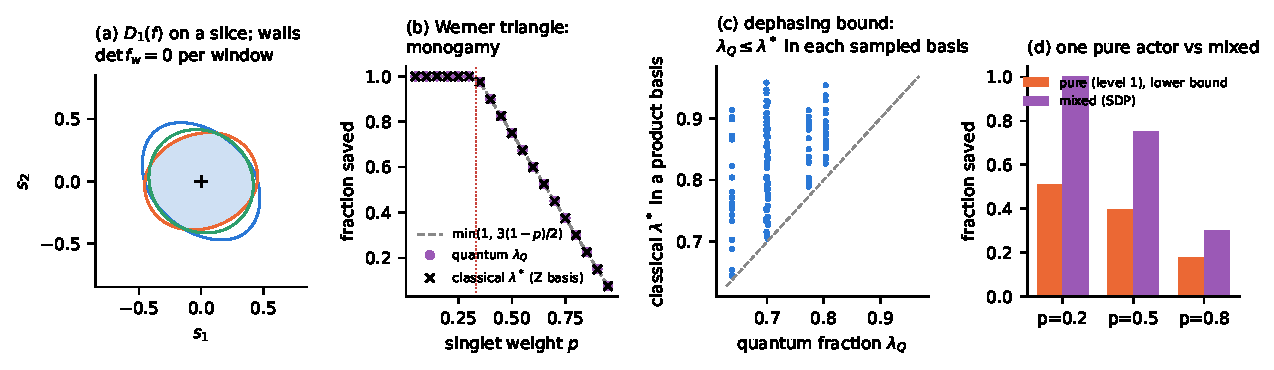
\includegraphics[width=\linewidth]{fig_qglue.pdf}
\caption{(a) A real two-dimensional slice of the pure domain $\mathcal D_1(f)$ for three random pairwise windows on three qubits: star-shaped
about $0$, bounded by pieces of the walls $\det f_w=0$ (one colour per window). (b) Pairwise Werner windows: the quantum fraction, the
formula $\min(1,\frac32(1-p))$ and the $Z$-basis classical $\lambda^*$; full gluing only for $p\le\frac13$. (c) The dephasing bound: for six
random quantum families, $\lambda^*$ in twenty random product bases against $\lambda_Q$, all above the diagonal. (d) The best pure
single-actor fraction (a lower bound) against the mixed fraction for Werner windows.}\label{fig:qglue}
\end{figure}

\section{A categorical home}\label{sec:categorical}

The previous sections left several structures without a common setting: the cover of contexts derived from commutators, the gauge of masked
measurements, the quantum rung without a fixed dimension, the information geometry, and the question of which dimension, if any, explains the
data. This section places them in one framework. It does not resolve the open problems; it says where each one lives. All computations are in
\texttt{engine/check\_npa.py} (NP1--NP6).

\paragraph{Representation functors and their limits.}
For an algebra $A$ of observables and a commutative ring $B$, the representations $\mathrm{Rep}_n(A)(B)=\mathrm{Hom}(A,M_n(B))$ form a functor
represented by a commutative affine scheme, with $GL_n$ acting by change of basis; its quotient is described by trace rings
\cite{Procesi1976}. Kontsevich and Rosenberg proposed reading the geometry of $A$ through the family $\mathrm{Rep}_n(A)$ \cite{KontsevichRosenberg2000},
and its derived version is representation homology \cite{BerestFelderRamadoss2014}. Li replaces $M_n$ by an arbitrary finite-dimensional
coefficient algebra $M$, $\mathrm{Rep}_M(A)(B)=\mathrm{Hom}(A,M\otimes B)$, and shows that non-matrix coefficients (strictly upper triangular
$3\times3$ matrices) detect singularities of the quantum plane and the Jordan plane that every matrix coefficient misses \cite{Li2026}. Our
fixed-dimension framing of \cref{sec:noncomm}, and the linear gauge of \cref{sec:masked} (the subgroup of $GL_3$ fixing the known
directions), are instances of this functor. What fails at finite dimension is made precise by the following.

\begin{proposition}[holonomy against dimension; NP5]\label{prop:holdim}
Invertible $n\times n$ matrices with $UV=qVU$ exist iff $q^n=1$. Hence for $q=e^{2\pi ik/N}$ ($\gcd(k,N)=1$) they exist exactly when $N$
divides $n$, and for an irrational phase in no finite dimension; the corresponding algebra (the noncommutative torus) nevertheless has a rich
category of infinite-dimensional modules \cite{Rieffel1981,Connes1994}. The Weyl relation $xy-yx=1$ has no finite-dimensional solution at all.
\end{proposition}

\begin{proof}
Taking determinants, $\det U\det V=q^n\det V\det U$. Clock and shift matrices tensored with $I_{n/N}$ realise the relation when $N\mid n$.
For the Weyl relation take traces: $0=n$.
\end{proof}

So a loop that carries a phase incommensurable with every finite dimension leaves every $\mathrm{Rep}_n$ empty. Numerically, the best unitary
residual $\|UV-qVU\|$ is $7\times10^{-7}$ for $q^3=1$, $n=3$, and $1.41$, $1.04$ for $n=2,4$, and stays above $0.75$ for an irrational phase
(\cref{fig:npa}(c)). The physical instance is Tsirelson's problem: Slofstra built games whose perfect quantum strategies exist only in
infinite dimensions \cite{Slofstra2020}. This is a different phenomenon from the $\mathbb Z/2$ exchange of actors of \cref{sec:monodromy},
which lives at a fixed dimension.

\paragraph{The module category, with positivity.}
Gabriel and Rosenberg recover a scheme from its category of quasi-coherent sheaves \cite{Gabriel1962,Rosenberg1998}, and Artin and Zhang take
a category of graded modules as the definition of a noncommutative projective scheme \cite{ArtinZhang1994}. Taking the category of modules as
the space removes the dimension constraint above: infinite-dimensional modules are objects like any other. Two corrections are needed for
probability. First, a plain module category has no positivity, and every result of the ladder lives in a cone, so the right category is that
of $*$-representations on Hilbert spaces (or of operator systems). Second, a state is not an object but a pointed one: the GNS construction
turns a state into a cyclic $*$-representation with a distinguished vector. Observables are recovered as natural endomorphisms of the
forgetful functor, and the matrix polynomials of \cref{sec:qglue} are morphisms between free modules; their free locus is the set of modules
on which such a morphism fails to be invertible.

This is also what makes the framework computable. The NPA hierarchy \cite{NPA2007,NPA2008} builds the GNS module from words in the
observables, truncated by length, and imposes positivity of its moment matrix; no dimension is fixed. It reproduces Tsirelson's bound
$2\sqrt2$ at levels $1$, $1{+}AB$ and $2$ (NP1), and it gives the dimension-free quantum rung directly on tables: the largest $\lambda$ with
$\lambda q\le P$ cellwise for a quantum behaviour $q$.

\begin{proposition}[the rungs on isotropic boxes; NP2, NP3]\label{prop:iso}
For the box with correlators $\pm v$ and unbiased marginals, $\tfrac12\le v\le1$: the classical fraction is $\lambda^*=2(1-v)$, and the quantum
fraction is $1$ for $v\le1/\sqrt2$ and $(1-v)/(1-1/\sqrt2)$ beyond.
\end{proposition}

\begin{proof}
Write the box as $\lambda q+(1-\lambda)r$ with $r$ no-signalling. The CHSH value is linear, equal to $4v$ for the box, at most $2$ for local $q$,
at most $2\sqrt2$ for quantum $q$ and at most $4$ for $r$; so $4v\le2\lambda+4(1-\lambda)$, i.e.\ $\lambda\le2(1-v)$, and $4v\le2\sqrt2\lambda+
4(1-\lambda)$, i.e.\ $\lambda\le(1-v)/(1-1/\sqrt2)$. Both bounds are attained, by local deterministic boxes and by the Tsirelson box,
respectively, mixed with the PR box.
\end{proof}

The engine's linear program and NPA reproduce both formulas at $21$ values of $v$ to $4\times10^{-10}$ (\cref{fig:npa}(a)); on random
no-signalling boxes the hierarchy is ordered, $\lambda^*\le\lambda_{\mathrm{NPA}(2)}\le\lambda_{\mathrm{NPA}(1+AB)}\le\lambda_{\mathrm{NPA}(1)}\le1$
(\cref{fig:npa}(b)). For two parties with two-outcome measurements, Jordan's lemma reduces quantum correlations to qubits, so here the
dimension-free rung adds nothing beyond $\mathrm{Rep}_2$; it matters where \cref{prop:holdim} bites.

\paragraph{Contexts as a diagram, contextuality as a failed limit.}
De~Silva and Barbosa associate to an operator algebra the diagram of Gelfand spectra of its commutative subalgebras (the spectral presheaf of
Isham, Butterfield and Hamilton \cite{IshamButterfield1998}), and extend any functor on spaces to all algebras by taking the limit over that
diagram \cite{deSilvaBarbosa2019}. The diagram is our commutation cover. Kochen--Specker \cite{KochenSpecker1967} says its limit of points is
empty; Gleason \cite{Gleason1957} says compatible probability assignments still exist. Contextuality sits between the two: probabilities agree
across contexts but come from no measure on global points, and $\lambda^*$ measures how far.

\begin{proposition}[Peres--Mermin; NP6]\label{prop:pm}
For the nine two-qubit Pauli observables of the Peres--Mermin square \cite{Peres1990,Mermin1990}, the commutation cliques are the six lines; no
$\pm1$ assignment respects all six line products; and for every state the six context tables agree on overlaps (a signed global section exists)
while $\lambda^*=0$.
\end{proposition}

\begin{proof}
Five line products are $+I$ and one is $-I$, so the product of all six constraints over the nine values is $+1=-1$. Every global assignment
therefore violates some line, where it hits a cell of probability zero, so any sub-measure below the tables vanishes. The tables come from one
state on jointly measurable sets, so they agree on overlaps.
\end{proof}

Checked for the maximally mixed state and five random states (rung $\R$, $\lambda^*=0$, linear gap $0$). This is state-independent
contextuality, the cleanest case where points collapse but probabilities survive.

\paragraph{Information geometry as enrichment.}
Perrone enriches Markov categories (states as morphisms out of the unit, channels as morphisms) in divergences, so that composition and tensor
can only contract them; data processing inequalities follow from the enrichment \cite{Perrone2023,Fritz2020}. For gluing it gives the following.

\begin{proposition}[data processing for gluing; NP4]\label{prop:dpi}
Applying local channels to the outcomes of each variable never decreases $\lambda^*$.
\end{proposition}

\begin{proof}
Push the optimal sub-measure $\mu$ (with $\mu|_w\le t_w$) through the channels. Positivity of the channels keeps every marginal below the
processed tables, and the mass is unchanged.
\end{proof}

Processing the evidence cannot create contextuality, consistent with the monotones of Abramsky, Barbosa and Mansfield
\cite{AbramskyBarbosaMansfield2017}. On ten random boxes the level-$(1{+}AB)$ quantum fraction never decreased either (numerical, not
proved). A quantum Markov category has no copy map, and that failure of copying is non-commutativity itself.

\begin{table}[!htbp]\centering\small
\begin{tabular}{p{0.3\linewidth}p{0.62\linewidth}}\toprule
earlier structure & categorical home\\\midrule
cover of contexts (\cref{sec:noncomm}) & the diagram of commutative subalgebras (spectral presheaf)\\
gluing and its failure (\cref{sec:graded,sec:ladder}) & limits over that diagram: points (Kochen--Specker) versus probabilities (Gleason)\\
the ladder of rungs & the cone in which the sections live: orthant, positive semidefinite, signed, complex\\
quantum rung without fixed dimension & positivity on truncated free modules (NPA)\\
masked directions, gauge (\cref{sec:masked}) & the $GL_n$ action on $\mathrm{Rep}_n(A)$ and its quotient\\
holonomy and phases (\cref{sec:noncomm}) & relations such as $UV=qVU$; finite dimension only when $q^n=1$\\
positivity domains (\cref{sec:qglue}) & morphisms of free modules; free loci as non-invertibility\\
information geometry & divergence-enriched Markov categories; data processing\\\midrule
level-two latent strata, flattening, hyperdeterminant & remain commutative algebraic geometry\\
Werner formula, quantum slices & open\\\bottomrule
\end{tabular}
\caption{What the categorical view gives a home to, and what it does not.}\label{tab:cat}
\end{table}

\Cref{tab:cat} summarises the placement. The categorical view unifies the framework; it does not by itself compute anything, which is why the
NPA truncation matters, and it leaves the commutative level-two results and the open problems where they were.

\begin{figure}[!htbp]\centering
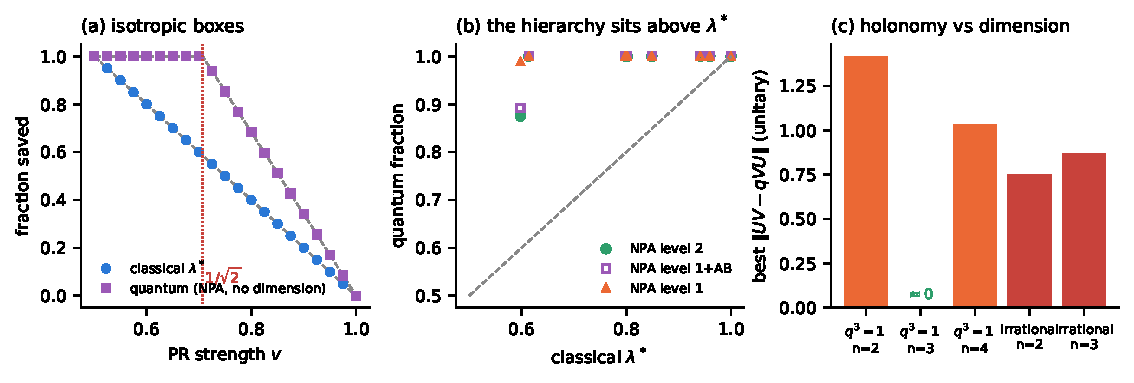
\includegraphics[width=\linewidth]{fig_npa.pdf}
\caption{(a) Isotropic PR boxes: the classical fraction $\lambda^*=2(1-v)$ and the dimension-free quantum fraction (NPA level $1{+}AB$), $1$ up to
$v=1/\sqrt2$ and $(1-v)/(1-1/\sqrt2)$ beyond (dashed: \cref{prop:iso}). (b) Twelve random no-signalling boxes: the quantum fraction at three
levels against $\lambda^*$. (c) The best unitary residual of $UV=qVU$ by dimension: zero only when $q^n=1$
(\cref{prop:holdim}).}\label{fig:npa}
\end{figure}

\section{What this says about probability built on schemes}\label{sec:summary}

\begin{table}[!htbp]\centering\small
\begin{tabular}{p{0.32\linewidth}p{0.6\linewidth}}\toprule
probabilistic notion & geometric form\\\midrule
the tables glue & $\lambda^*=1$: the level-one fibre (a polytope) is non-empty\\
graded partial gluing & the slices $E_\alpha$ of the polytope $\{\mu\ge0:\mu|_w\le t_w\}$, $0<\alpha\le\lambda^*$\\
dissipated mass & the residues $r_w$ of \eqref{eq:split}; $1-\alpha$ of every table\\
most probable path & the entropy maximisers $q_\alpha$, continuous in $\alpha$\\
latent actors & the fibre $\mathcal X_P$ of the polynomial map $F$, an affine scheme\\
actors merge, or one is absent & singular strata; over an independent law, the Stanley--Reisner scheme of a simplicial complex\\
actors partly invisible & the non-flat locus $\{w_1w_2d_1d_2d_3=0\}$ ($m=3$)\\
second-order obstruction ($\ell_2\neq0$) & $\kappa=C^\top D^2F$; tangent cone = union of branches\\
abrupt change & a path of laws crossing a fold of the image; Puiseux branches $\pm\sqrt s$\\
a structure dies, a new one is born & real points of the fibre become a complex-conjugate pair (sign of the hyperdeterminant); three types fit\\
signed mixtures & real points with weights outside $[0,1]$ ($\mathrm{Det}>0>\Delta_m$)\\
kinds of incoherence & rungs of the ladder $\mathbb C\supset\R\supset\R_{\ge0}$: no points (direct influence), $\R$ not $\R_{\ge0}$ (contextuality, negativity $\nu$), $\mathbb C$ not $\R$ (level two)\\
commutation obstruction & the cover of contexts; order effects $\le\|[P,Q]\|$; Kirkwood--Dirac section on the $\mathbb C$ rung\\
loops of evidence & geometric phase; non-abelian holonomy with rank-two projections\\
masked measurements & linear ambiguity of dimension $\max(0,3(3-\dim V)-h)$; the cone culls candidates implying negative probabilities; recoverable = invariants of the residual group\\
categorical home & contexts as a diagram of commutative subalgebras; contextuality as a failed limit; NPA truncation; $q^n=1$ obstruction; data processing\\
quantum rung & positivity domain of $\bigoplus_w(\rho_w^\top-K_w^*K_w)$; walls in the free locus $\det f_w=0$; $\lambda_Q\le\lambda^*$ in every product basis\\
probability paths & Zeno dragging: success $\cos^{4jN}(\Theta/2N)\to1$, only with non-commuting projections\\
dual roles & monodromy of $F$ (a subgroup of $S_k$); trivial on real mixtures when $m=3$ because the non-flat walls separate the sheets\\\bottomrule
\end{tabular}
\caption{The dictionary.}\label{tab:dict}
\end{table}

\Cref{tab:dict} collects the dictionary. Level one is linear: explanations form polytopes, the gradation $\alpha$ slices them, and
everything is a linear program. The only way the structure changes is through the combinatorics of the slices. Level two is polynomial:
explanations are the real points of the fibres of $F$, the fibres have singular points where the actors merge or vanish, the
obstruction to deforming an explanation is quadratic, and closed loops of evidence can permute the actors. The gradation lives at both
levels ($\lambda^*$ and $\lambda^*_2$), and so a programme for a theory of probability on schemes is: for each level, the fibre over the
evidence; for each fibre, its graded slices; and for each path of evidence, the path it induces through the slices, including where it
must pass through a singularity and what is lost or born there.

\paragraph{Related work.}
The noncontextual fraction and the sheaf view of local tables are due to Abramsky and coauthors \cite{AbramskyBrandenburger2011,AbramskyBarbosaMansfield2017}; graded agreement in sheaves of pseudometric spaces is Robinson's consistency radius \cite{Robinson2020}; the companion report \cite{Main} develops the level-one engine. That latent-class and other hidden-variable models are stratified, singular algebraic families is classical in algebraic statistics \cite{GeigerEtAl2001,PachterSturmfels2005}, and the consequences of their singularities for estimation and testing are studied by Drton \cite{Drton2009} and Watanabe \cite{Watanabe2009}. Generic identifiability of two-type models on three or more binary variables is due to Allman, Matias and Rhodes \cite{AllmanMatiasRhodes2009}. The secant-cumulant coordinates of \cref{sec:scheme} and the toric structure of secant varieties are due to Michałek, Oeding and Zwiernik \cite{MichalekOedingZwiernik2015}; the semialgebraic description of tensors of nonnegative rank two to Allman, Rhodes, Sturmfels and Zwiernik \cite{AllmanRhodesSturmfelsZwiernik2015}, with a book-length treatment of semialgebraic latent models by Zwiernik \cite{Zwiernik2016}; real rank and the hyperdeterminant to de~Silva and Lim \cite{deSilvaLim2008} and Gelfand, Kapranov and Zelevinsky \cite{GelfandKapranovZelevinsky1994}; Stanley--Reisner theory and flatness are standard \cite{MillerSturmfels2005,Matsumura1986}. What we add is the combination: graded partial gluing at the failure of a sheaf condition, lifted to the level of hypotheses, with the singular strata, second-order obstruction, Puiseux crossing and monodromy read as what happens to latent actors when evidence moves.

\paragraph{Limits.}
The categorical section is a framework, not a theorem: its computations (NPA, the Peres--Mermin square, the $q^n=1$ obstruction, data
processing) are standard or elementary, and the monotonicity of the quantum fraction under processing is checked, not proved. The quantum section uses three qubits with pairwise windows; the Werner formula is computed and certified numerically, not proved; pure
fractions are lower bounds from a non-smooth optimisation; topology changes of the normalised quantum slices were not established, because
their maximisers come in continuous families. The masking study uses two qubits with random states and directions, six trials per level, and a Gaussian $\chi^2$ calibration that proved
somewhat optimistic; the positivity-only search samples the feasible set by random walks and does not certify its extent. The non-commutative section uses spin models and small random examples; its molecular reading is an analogy, not chemistry, and its
scheme-theoretic part (reducedness with coherences, the $\mathrm{Rep}_d$ tower) is stated, not computed. The exact scheme results are for two types: the Stanley--Reisner fibre for $m=3,4$, the closed form and the stratification for $m=3$, and
one flat point for $m=4$; the level-two ladder is for $m=3$, and the level-one comparability constants are measured, not derived, beyond
the upper bound. The fibres are semialgebraic (they carry the inequalities $w\ge0$, $0\le a\le1$, $\alpha F\le t$), so ``scheme'' is used for the
equations and the real points with these inequalities are the explanations. All variables are binary, and the level-two results are for
two types. The values of $\lambda_2^*$ and the level-two intervals come from multi-start optimisation and are certified only as
attained (lower bounds for $\lambda^*_2$, inner bounds for intervals); the regularity of the 4-variable loop is checked at 500 points,
not proved. The examples are synthetic with exact tables: there is no sampling error, and no real trial data were used.

\paragraph{Next steps.}
(1) Certified level-two bounds by polynomial optimisation (moment and sum-of-squares relaxations), which would give upper bounds on
$\lambda^*_2$ to match the lower ones. (2) The images of the three-type model and their folds: where the third actor of
\cref{sec:puiseux} is itself forced to merge or vanish. (3) Monodromy for $k\ge3$ (subgroups of $S_k$) and its relation to the
singular strata. (4) A pre-registered test on aggregated combination-trial tables, if published pair and triple tables can be found;
nothing patient-level would be needed. (5) Schemes that see positivity: over $\R$ or $\mathbb C$ the linear equations of level one always
have solutions when the tables agree on overlaps, so contextuality is invisible to ordinary schemes; it is a statement about
$\R_{\ge0}$-points. Semiring schemes (blueprints \cite{Lorscheid2012}, tropical schemes \cite{GiansiracusaGiansiracusa2016}) are the
natural home for gluing with positivity, with $\lambda^*$ and the graded explanations as their points over the $\alpha$-line.
(6) The flattening stratification for $m\ge4$ and $k\ge3$. (7) Non-commutative level two: whether the fibre over a merge point stays reduced once coherences are allowed (qubit actors), the
quantum rung by the NPA hierarchy alongside $\lambda^*$, and whether laws on the complex rung of \cref{sec:ladder} have qubit-actor
explanations. (8) A pre-registered order-effect test (the QQ equality and the commutator bound) on aggregated survey data. (9) The quantum slices:
topology of the normalised explanation sets as the evidence moves (the analogue of Example~4.3 of \cite{IVW2026}), with continuous
symmetries quotiented out; an analytic proof of the Werner formula; and the meaning of the higher levels of the free domain. (10) A scenario where the module level genuinely exceeds every
fixed dimension (multi-outcome or multipartite, or a Slofstra-type game), and representation homology with non-matrix coefficients
\cite{Li2026} as a test of where finite explanations become singular.

\paragraph{Reproducibility.}
The engine module is \texttt{engine/pce/level2.py}; \texttt{engine/check\_level2.py} runs nine checks (LV1--LV9: graded explanations,
the conflicting trials, the exact second derivative, the strata, the tangent cone, the Puiseux crossing, monodromy, sharpening, and level-two graded gluing) and
writes \texttt{level2/level2\_results.json}; \texttt{level2/fig\_level2.py} draws \cref{fig:main}. \texttt{engine/check\_scheme.py}
runs six exact symbolic checks (SC1--SC6: the moment normal form, the Stanley--Reisner fibre and its primary decomposition, the closed-form
inverse and Jacobian, the hyperdeterminant, the $m=3$ strata, and the flat point for $m=4$) in a few seconds and writes
\texttt{level2/scheme\_results.json}; \texttt{level2/fig\_scheme.py} draws \cref{fig:scheme}. The exploratory scripts are in
\texttt{level2/scheme/}. \texttt{engine/pce/ladder.py} computes the rungs and their measures; \texttt{engine/check\_ladder.py} runs six
checks (LD1--LD6) and writes \texttt{level2/ladder\_results.json}; \texttt{level2/fig\_ladder.py} draws \cref{fig:ladder}.
\texttt{engine/pce/noncomm.py} implements spin rotations, sequential measurement, the commutation cover, the Kirkwood--Dirac section,
Bargmann invariants and Zeno dragging; \texttt{engine/check\_noncomm.py} runs eight checks (NC1--NC8) and writes
\texttt{level2/noncomm\_results.json}; \texttt{level2/fig\_noncomm.py} draws \cref{fig:noncomm}.
\texttt{engine/pce/masked.py} implements the two-qubit tables, the linear and positivity-constrained fits, the lattice culls, sweeps and
the feasible-region search; \texttt{engine/check\_masked.py} (MK1--MK6, about 13 minutes) writes \texttt{level2/masked\_results.json},
\texttt{engine/check\_masked\_gauge.py} (MK7) checks the dimension formula, and \texttt{level2/fig\_masked.py} draws \cref{fig:masked}.
\texttt{engine/pce/qglue.py} builds the hereditary quadratics, their linearisations and the pure and mixed quantum fractions (semidefinite
programs solved with SCS through cvxpy); \texttt{engine/check\_qglue.py} (QG1--QG6) writes \texttt{level2/qglue\_results.json};
\texttt{level2/fig\_qglue.py} draws \cref{fig:qglue}.
\texttt{engine/pce/npa.py} implements the NPA levels $1$, $1{+}AB$ and $2$ for bipartite binary scenarios and the dimension-free quantum
fraction; \texttt{engine/check\_npa.py} (NP1--NP6) writes \texttt{level2/npa\_results.json}; \texttt{level2/fig\_npa.py} draws \cref{fig:npa}.

\begin{thebibliography}{99}\small
\bibitem{AbramskyBrandenburger2011} S.~Abramsky and A.~Brandenburger, The sheaf-theoretic structure of non-locality and
  contextuality. \emph{New J. Phys.} \textbf{13} (2011), 113036.
\bibitem{AbramskyBrandenburger2014} S.~Abramsky and A.~Brandenburger, An operational interpretation of negative probabilities and
  no-signalling models. In \emph{Horizons of the Mind}, Lecture Notes in Computer Science \textbf{8464}, Springer, 2014;
  arXiv:1401.2561.
\bibitem{AbramskyBarbosaMansfield2017} S.~Abramsky, R.~S. Barbosa and S.~Mansfield, Contextual fraction as a measure of
  contextuality. \emph{Phys. Rev. Lett.} \textbf{119} (2017), 050504.
\bibitem{AllmanMatiasRhodes2009} E.~S. Allman, C.~Matias and J.~A. Rhodes, Identifiability of parameters in latent structure models with
  many observed variables. \emph{Ann. Statist.} \textbf{37} (2009), 3099--3132.
\bibitem{Berge1963} C.~Berge, \emph{Topological Spaces}. Oliver and Boyd, 1963.
\bibitem{BurkeFerris1993} J.~V. Burke and M.~C. Ferris, Weak sharp minima in mathematical programming. \emph{SIAM J. Control
  Optim.} \textbf{31} (1993), 1340--1359.
\bibitem{Drton2009} M.~Drton, Likelihood ratio tests and singularities. \emph{Ann. Statist.} \textbf{37} (2009), 979--1012.
\bibitem{GeigerEtAl2001} D.~Geiger, D.~Heckerman, H.~King and C.~Meek, Stratified exponential families: graphical models and model
  selection. \emph{Ann. Statist.} \textbf{29} (2001), 505--529.
\bibitem{PachterSturmfels2005} L.~Pachter and B.~Sturmfels (eds.), \emph{Algebraic Statistics for Computational Biology}. Cambridge
  University Press, 2005.
\bibitem{PopescuRohrlich1994} S.~Popescu and D.~Rohrlich, Quantum nonlocality as an axiom. \emph{Found. Phys.} \textbf{24}
  (1994), 379--385.
\bibitem{Robinson2020} M.~Robinson, Assignments to sheaves of pseudometric spaces. \emph{Compositionality} \textbf{2} (2020);
  doi:10.32408/compositionality-2-2.
\bibitem{AllmanRhodesSturmfelsZwiernik2015} E.~S. Allman, J.~A. Rhodes, B.~Sturmfels and P.~Zwiernik, Tensors of nonnegative rank two.
  \emph{Linear Algebra Appl.} (2015); arXiv:1305.0539.
\bibitem{CasasAlvero2000} E.~Casas-Alvero, \emph{Singularities of Plane Curves}. London Mathematical Society Lecture Note Series
  \textbf{276}, Cambridge University Press, 2000.
\bibitem{CHSH1969} J.~F. Clauser, M.~A. Horne, A.~Shimony and R.~A. Holt, Proposed experiment to test local hidden-variable theories.
  \emph{Phys. Rev. Lett.} \textbf{23} (1969), 880--884.
\bibitem{CoxLittleOShea2015} D.~A. Cox, J.~Little and D.~O'Shea, \emph{Ideals, Varieties, and Algorithms}, 4th ed. Springer, 2015.
\bibitem{deSilvaLim2008} V.~de~Silva and L.-H. Lim, Tensor rank and the ill-posedness of the best low-rank approximation problem.
  \emph{SIAM J. Matrix Anal. Appl.} \textbf{30} (2008), 1084--1127.
\bibitem{GelfandKapranovZelevinsky1994} I.~M. Gelfand, M.~M. Kapranov and A.~V. Zelevinsky, \emph{Discriminants, Resultants, and
  Multidimensional Determinants}. Birkh\"auser, 1994.
\bibitem{GiansiracusaGiansiracusa2016} J.~Giansiracusa and N.~Giansiracusa, Equations of tropical varieties. \emph{Duke Math. J.}
  \textbf{165} (2016), 3379--3433.
\bibitem{Kuranishi1962} M.~Kuranishi, On the locally complete families of complex analytic structures. \emph{Ann. of Math.}
  \textbf{75} (1962), 536--577.
\bibitem{LadaStasheff1993} T.~Lada and J.~Stasheff, Introduction to sh Lie algebras for physicists. \emph{Internat. J. Theoret. Phys.}
  \textbf{32} (1993), 1087--1103.
\bibitem{Landsberg2012} J.~M. Landsberg, \emph{Tensors: Geometry and Applications}. Graduate Studies in Mathematics \textbf{128},
  American Mathematical Society, 2012.
\bibitem{Lorscheid2012} O.~Lorscheid, The geometry of blueprints. Part I. \emph{Adv. Math.} \textbf{229} (2012), 1804--1846.
\bibitem{Matsumura1986} H.~Matsumura, \emph{Commutative Ring Theory}. Cambridge University Press, 1986.
\bibitem{MichalekOedingZwiernik2015} M.~Michałek, L.~Oeding and P.~Zwiernik, Secant cumulants and toric geometry. \emph{Int. Math. Res.
  Not.} (2015); arXiv:1212.1515.
\bibitem{MillerSturmfels2005} E.~Miller and B.~Sturmfels, \emph{Combinatorial Commutative Algebra}. Graduate Texts in Mathematics
  \textbf{227}, Springer, 2005.
\bibitem{Zwiernik2016} P.~Zwiernik, \emph{Semialgebraic Statistics and Latent Tree Models}. Chapman and Hall/CRC, 2016.
\bibitem{DzhafarovKujala2016} E.~N. Dzhafarov and J.~V. Kujala, Context--content systems of random variables: the
  contextuality-by-default theory. \emph{J. Math. Psych.} \textbf{74} (2016), 11--33.
\bibitem{Hoffman1952} A.~J. Hoffman, On approximate solutions of systems of linear inequalities. \emph{J. Res. Nat. Bur. Standards}
  \textbf{49} (1952), 263--265.
\bibitem{SymPy2017} A.~Meurer et al., SymPy: symbolic computing in Python. \emph{PeerJ Comput. Sci.} \textbf{3} (2017), e103.
\bibitem{Watanabe2009} S.~Watanabe, \emph{Algebraic Geometry and Statistical Learning Theory}. Cambridge University Press, 2009.
\bibitem{Main} V.~K. Awasthi, The Posterior Coherence Engine: separating uncertainty from incoherence. Technical report, October 2026.
\bibitem{AharonovVardi1980} Y.~Aharonov and M.~Vardi, Meaning of an individual ``Feynman path''. \emph{Phys. Rev. D} \textbf{21} (1980), 2235.
\bibitem{ArvidssonShukur2024} D.~R.~M. Arvidsson-Shukur et al., Properties and applications of the Kirkwood--Dirac distribution.
  \emph{New J. Phys.} (2024); arXiv:2403.18899.
\bibitem{Bargmann1964} V.~Bargmann, Note on Wigner's theorem on symmetry operations. \emph{J. Math. Phys.} \textbf{5} (1964), 862--868.
\bibitem{Berry1984} M.~V. Berry, Quantal phase factors accompanying adiabatic changes. \emph{Proc. R. Soc. Lond. A} \textbf{392} (1984), 45--57.
\bibitem{Dirac1945} P.~A.~M. Dirac, On the analogy between classical and quantum mechanics. \emph{Rev. Mod. Phys.} \textbf{17} (1945), 195--199.
\bibitem{Halmos1969} P.~R. Halmos, Two subspaces. \emph{Trans. Amer. Math. Soc.} \textbf{144} (1969), 381--389.
\bibitem{Kirkwood1933} J.~G. Kirkwood, Quantum statistics of almost classical assemblies. \emph{Phys. Rev.} \textbf{44} (1933), 31--37.
\bibitem{LeBruyn2008} L.~Le~Bruyn, \emph{Noncommutative Geometry and Cayley-smooth Orders}. Chapman and Hall/CRC, 2008.
\bibitem{Luders1951} G.~L\"uders, \"Uber die Zustands\"anderung durch den Me\ss prozess. \emph{Ann. Phys.} \textbf{443} (1951), 322--328.
\bibitem{MIPRE2020} Z.~Ji, A.~Natarajan, T.~Vidick, J.~Wright and H.~Yuen, MIP$^*$ = RE. arXiv:2001.04383, 2020.
\bibitem{MisraSudarshan1977} B.~Misra and E.~C.~G. Sudarshan, The Zeno's paradox in quantum theory. \emph{J. Math. Phys.} \textbf{18} (1977), 756--763.
\bibitem{NPA2007} M.~Navascu\'es, S.~Pironio and A.~Ac\'in, Bounding the set of quantum correlations. \emph{Phys. Rev. Lett.} \textbf{98} (2007), 010401.
\bibitem{Pancharatnam1956} S.~Pancharatnam, Generalized theory of interference and its applications. \emph{Proc. Indian Acad. Sci. A}
  \textbf{44} (1956), 247--262.
\bibitem{Procesi1976} C.~Procesi, The invariant theory of $n\times n$ matrices. \emph{Adv. Math.} \textbf{19} (1976), 306--381.
\bibitem{Pusey2014} M.~F. Pusey, Anomalous weak values are proofs of contextuality. \emph{Phys. Rev. Lett.} \textbf{113} (2014), 200401.
\bibitem{Slofstra2019} W.~Slofstra, The set of quantum correlations is not closed. \emph{Forum Math. Pi} \textbf{7} (2019), e1.
\bibitem{Tsirelson1980} B.~S. Cirel'son, Quantum generalizations of Bell's inequality. \emph{Lett. Math. Phys.} \textbf{4} (1980), 93--100.
\bibitem{WangBusemeyer2014} Z.~Wang, T.~Solloway, R.~M. Shiffrin and J.~R. Busemeyer, Context effects produced by question orders reveal
  quantum nature of human judgments. \emph{Proc. Natl. Acad. Sci. USA} \textbf{111} (2014), 9431--9436.
\bibitem{WilczekZee1984} F.~Wilczek and A.~Zee, Appearance of gauge structure in simple dynamical systems. \emph{Phys. Rev. Lett.}
  \textbf{52} (1984), 2111--2114.
\bibitem{BasuPollackRoy2006} S.~Basu, R.~Pollack and M.-F. Roy, \emph{Algorithms in Real Algebraic Geometry}, 2nd ed. Springer, 2006.
\bibitem{Horodecki1995} R.~Horodecki, P.~Horodecki and M.~Horodecki, Violating Bell inequality by mixed spin-$\frac12$ states: necessary
  and sufficient condition. \emph{Phys. Lett. A} \textbf{200} (1995), 340--344.
\bibitem{Peres1996} A.~Peres, Separability criterion for density matrices. \emph{Phys. Rev. Lett.} \textbf{77} (1996), 1413--1415.
\bibitem{IVW2026} A.~Islam, J.~Volčič and H.~J. Woerdeman, Positivity of hereditary quadratic NC polynomials and $x^*x$-convex domains.
  arXiv:2610.14053, 2026.
\bibitem{JKMMP2021} M.~Jury, I.~Klep, M.~E. Mancuso, S.~McCullough and J.~E. Pascoe, Noncommutative partial convexity via $\Gamma$-convexity.
  \emph{J. Geom. Anal.} \textbf{31} (2021), 3137--3160.
\bibitem{ArtinZhang1994} M.~Artin and J.~J. Zhang, Noncommutative projective schemes. \emph{Adv. Math.} \textbf{109} (1994), 228--287.
\bibitem{BerestFelderRamadoss2014} Yu.~Berest, G.~Felder and A.~Ramadoss, Derived representation schemes and noncommutative geometry. In
  \emph{Expository Lectures on Representation Theory}, Contemp. Math. \textbf{607}, Amer. Math. Soc., 2014, 113--162.
\bibitem{Connes1994} A.~Connes, \emph{Noncommutative Geometry}. Academic Press, 1994.
\bibitem{deSilvaBarbosa2019} N.~de~Silva and R.~S. Barbosa, Contextuality and noncommutative geometry in quantum mechanics. \emph{Comm. Math.
  Phys.} \textbf{365} (2019), 375--429.
\bibitem{Fritz2020} T.~Fritz, A synthetic approach to Markov kernels, conditional independence and theorems on sufficient statistics.
  \emph{Adv. Math.} \textbf{370} (2020), 107239.
\bibitem{Gabriel1962} P.~Gabriel, Des cat\'egories ab\'eliennes. \emph{Bull. Soc. Math. France} \textbf{90} (1962), 323--448.
\bibitem{Gleason1957} A.~M. Gleason, Measures on the closed subspaces of a Hilbert space. \emph{J. Math. Mech.} \textbf{6} (1957), 885--893.
\bibitem{IshamButterfield1998} C.~J. Isham and J.~Butterfield, A topos perspective on the Kochen--Specker theorem: I. Quantum states as
  generalized valuations. \emph{Internat. J. Theoret. Phys.} \textbf{37} (1998), 2669--2733.
\bibitem{KochenSpecker1967} S.~Kochen and E.~P. Specker, The problem of hidden variables in quantum mechanics. \emph{J. Math. Mech.}
  \textbf{17} (1967), 59--87.
\bibitem{KontsevichRosenberg2000} M.~Kontsevich and A.~L. Rosenberg, Noncommutative smooth spaces. In \emph{The Gelfand Mathematical Seminars,
  1996--1999}, Birkh\"auser, 2000, 85--108.
\bibitem{Li2026} G.~Li, Derived representation schemes with arbitrary coefficients and associative smoothness. arXiv:2607.19654, 2026.
\bibitem{Mermin1990} N.~D. Mermin, Simple unified form for the major no-hidden-variables theorems. \emph{Phys. Rev. Lett.} \textbf{65} (1990),
  3373--3376.
\bibitem{NPA2008} M.~Navascu\'es, S.~Pironio and A.~Ac\'in, A convergent hierarchy of semidefinite programs characterizing the set of quantum
  correlations. \emph{New J. Phys.} \textbf{10} (2008), 073013.
\bibitem{Peres1990} A.~Peres, Incompatible results of quantum measurements. \emph{Phys. Lett. A} \textbf{151} (1990), 107--108.
\bibitem{Perrone2023} P.~Perrone, Categorical information geometry. In \emph{Geometric Science of Information (GSI 2023)}, Lecture Notes in
  Computer Science, Springer, 2023.
\bibitem{Rieffel1981} M.~A. Rieffel, C$^*$-algebras associated with irrational rotations. \emph{Pacific J. Math.} \textbf{93} (1981), 415--429.
\bibitem{Rosenberg1998} A.~L. Rosenberg, The spectrum of abelian categories and reconstruction of schemes. In \emph{Rings, Hopf Algebras, and
  Brauer Groups}, Lecture Notes in Pure and Appl. Math. \textbf{197}, Dekker, 1998, 257--274.
\bibitem{Slofstra2020} W.~Slofstra, Tsirelson's problem and an embedding theorem for groups arising from non-local games. \emph{J. Amer. Math.
  Soc.} \textbf{33} (2020), 1--56.
\end{thebibliography}
\end{document}
